\documentclass[a4paper]{article}
\usepackage{vntex}
\usepackage{a4wide}
\usepackage{graphicx}
\usepackage{array}
\usepackage{tabularx}
\usepackage{multirow}
\usepackage[framemethod=tikz]{mdframed}
\usepackage{geometry}
\usepackage{setspace}
\usepackage{fancyhdr}
\usepackage{float}
\usepackage{longtable}
\usepackage{tocloft}
\usepackage{tikz}
\usetikzlibrary{calc}
\usepackage{amsmath}
\usepackage{amssymb}
\usepackage{fvextra}
\usepackage{newunicodechar}
\usepackage{caption}
\usepackage[colorlinks=true, urlcolor=blue, linkcolor=black, citecolor=black, unicode=true]{hyperref}
\usepackage{xurl}
\renewcommand{\baselinestretch}{1.5}
\renewcommand{\figurename}{Hình}
\renewcommand{\tablename}{Bảng}
\renewcommand{\contentsname}{Mục lục}
\renewcommand{\refname}{Tài liệu tham khảo}
\setcounter{tocdepth}{2}
\captionsetup{labelsep=period}

% Sơ đồ (lưu đồ, sơ đồ quy trình) đánh số riêng, không chung với Hình
\floatstyle{plaintop}
\newfloat{sodo}{htbp}{los}
\floatname{sodo}{Sơ đồ}

% Ký tự Unicode ngoài bảng mã tiếng Việt
\newunicodechar{←}{\ensuremath{\leftarrow}}
\newunicodechar{→}{\ensuremath{\rightarrow}}
\newunicodechar{≤}{\ensuremath{\leq}}
\newunicodechar{≥}{\ensuremath{\geq}}
\newunicodechar{≠}{\ensuremath{\neq}}
\newunicodechar{∅}{\ensuremath{\emptyset}}
\newunicodechar{∈}{\ensuremath{\in}}
\newunicodechar{∉}{\ensuremath{\notin}}
\newunicodechar{∞}{\ensuremath{\infty}}
\newunicodechar{×}{\ensuremath{\times}}
\newunicodechar{·}{\ensuremath{\cdot}}
\newunicodechar{−}{\ensuremath{-}}
\newunicodechar{✓}{\ensuremath{\checkmark}}
\newunicodechar{₀}{\ensuremath{_0}}
\newunicodechar{₁}{\ensuremath{_1}}
\newunicodechar{₂}{\ensuremath{_2}}
\newunicodechar{²}{\ensuremath{^2}}
\newunicodechar{…}{\ldots}
\newunicodechar{—}{---}
\newunicodechar{–}{--}

% Căn giữa tiêu đề Mục lục
\renewcommand{\cfttoctitlefont}{\hfill\Large\bfseries}
\renewcommand{\cftaftertoctitle}{\hfill}

% Thiết lập Header và Footer
\setlength{\headheight}{40pt}
\pagestyle{fancy}
\fancyhead{}
\fancyhead[L]{
    {\setlength{\tabcolsep}{0pt}
    \begin{tabular}{rl}
        \begin{picture}(25,15)(0,0)
            \put(0,-8){
\includegraphics[width=8mm, height=8mm]{images/logo.png}}
        \end{picture} &
        \hspace{5pt}
        \begin{tabular}{l}
            \textbf{\ttfamily Trường Đại học Khoa học Tự nhiên, ĐHQG-HCM}\\
        \end{tabular}
    \end{tabular}}
}
\fancyhead[R]{}

\fancyfoot{}
\fancyfoot[L]{\scriptsize \ttfamily Cơ sở Trí tuệ Nhân tạo}
\fancyfoot[R]{\scriptsize \ttfamily Trang {\thepage}}
\renewcommand{\headrulewidth}{0.3pt}
\renewcommand{\footrulewidth}{0.3pt}

\begin{document}

% 1. Trang bìa
\begin{titlepage}
% --- BẮT ĐẦU VẼ KHUNG TRANG TRÍ ---
\begin{tikzpicture}[remember picture, overlay]
    % 1. Định nghĩa các điểm góc của khung
    \coordinate (TopLeft) at ($(current page.north west) + (2cm,-2cm)$);
    \coordinate (BottomRight) at ($(current page.south east) + (-1.5cm,2cm)$);
    \coordinate (TopRight) at (TopLeft -| BottomRight);
    \coordinate (BottomLeft) at (TopLeft |- BottomRight);

    % 2. Vẽ khung chính (Nét đôi đậm)
    \draw[line width=2pt, double distance=2pt, color=blue!50!black] (TopLeft) rectangle (BottomRight);

    % 3. Vẽ khung phụ bên trong (Nét đơn mảnh, cách khung chính 3pt)
    \draw[line width=0.5pt, color=blue!50!black]
        ($(TopLeft)+(3pt,-3pt)$) rectangle ($(BottomRight)+(-3pt,3pt)$);

    % 4. Vẽ họa tiết trang trí ở 4 góc (Hình thoi)
    \foreach \corner in {TopLeft, TopRight, BottomLeft, BottomRight}
        \node[fill=blue!50!black, inner sep=0pt, minimum size=8pt, rotate=45] at (\corner) {};

    % Chấm trắng nhỏ giữa hình thoi
    \foreach \corner in {TopLeft, TopRight, BottomLeft, BottomRight}
        \node[fill=white, inner sep=0pt, minimum size=2pt, rotate=45] at (\corner) {};
\end{tikzpicture}
% --- KẾT THÚC VẼ KHUNG ---
\begin{center}
    % --- PHẦN 1: TÊN TRƯỜNG & LOGO ---
    \vspace*{-2.5cm}

    \textbf{\large ĐẠI HỌC QUỐC GIA THÀNH PHỐ HỒ CHÍ MINH}\\
    \textbf{\large TRƯỜNG ĐẠI HỌC KHOA HỌC TỰ NHIÊN}\\
    \textbf{\large KHOA CÔNG NGHỆ THÔNG TIN}\\

    \vspace{0.6cm}
    
\includegraphics[width=5cm]{images/logo.png}
    \vspace{0.6cm}

    % --- PHẦN 2: TÊN ĐỀ TÀI ---
    \begin{tabular}{c}
        \multicolumn{1}{c}{\textbf{{\Large BÁO CÁO ĐỒ ÁN 1}}}\\
        \multicolumn{1}{c}{\textbf{{\LARGE CƠ SỞ TRÍ TUỆ NHÂN TẠO}}}\\
        ~~\\
        \hline
        \\
        \multicolumn{1}{c}{\textbf{{\Large Đề tài:}}}\\
        \vspace{0.2cm}
        \parbox{14cm}{\centering \textbf{{\LARGE BLOXORZ SOLVER}}\\[4pt]
            \textbf{{\Large GIẢI TRÒ CHƠI BLOXORZ BẰNG CÁC THUẬT TOÁN TÌM KIẾM}}}\\
        \\
        \hline
    \end{tabular}

    \vspace{1cm}

    % --- PHẦN 3: THÔNG TIN (Lệch phải) ---
    \begin{flushright}
        \begin{tabular}{r l}
            \textbf{Giảng viên hướng dẫn:} & \textbf{Bùi Tiến Lên} \\
            \textbf{Giảng viên thực hành:} & \textbf{Nguyễn Thanh Tình} \\
            \textbf{Lớp:} & \textbf{24\_22} \\
            \textbf{Nhóm thực hiện:} & 1. Phan Chí Cao* -- 24120026 \\
            & 2. Trần Văn Đức -- 24120042 \\
            & 3. Võ Phùng Nhật Long -- 24120088 \\
            & 4. Lâm Duy Minh -- 24120091 \\
            & 5. Hoàng Trọng Nghĩa -- 24120103 \\
        \end{tabular}
    \end{flushright}

    \vfill
    % --- PHẦN 4: NGÀY THÁNG ---
    {\footnotesize Thành phố Hồ Chí Minh, 10/2026}

    \vspace{-2cm}

\end{center}
\end{titlepage}


\thispagestyle{empty}
\newpage

% 2. Phân công và đánh giá thành viên
\section{Lập kế hoạch và phân công}

\subsection{Phân công nhiệm vụ}

Dự án được chia theo mô-đun để năm thành viên làm song song. Phần lõi (trạng thái, bảng chuyển tư thế, giao diện bài toán) được hoàn thành trước, các phần còn lại dùng chung giao diện này.

{\renewcommand{\arraystretch}{1.25}
\begin{longtable}{|>{\raggedright\arraybackslash}p{0.221\linewidth}|>{\raggedright\arraybackslash}p{0.337\linewidth}|>{\raggedright\arraybackslash}p{0.337\linewidth}|}
\hline
\textbf{Thành viên} & \textbf{Mã nguồn} & \textbf{Báo cáo / Video} \\ \hline
\endhead
\hline
\endlastfoot
\textbf{Phan Chí Cao} (24120026, nhóm trưởng) & Kiến trúc tổng thể; \texttt{State} và bảng chuyển tư thế; giao diện \texttt{BloxorzProblem} (\texttt{successors}, \texttt{is\_\allowbreak{}goal}); định dạng màn chơi JSON và bộ đọc màn; tích hợp và kiểm tra mã nguồn của các thành viên & Hình thức hoá bài toán; phân công; tổng hợp báo cáo; đóng gói bài nộp \\ \hline
\textbf{Trần Văn Đức} (24120042) & Giao diện Pygame 3D: vẽ bàn và khối, chơi bằng phím, các nút New Game / Restart / chọn màn / Solve ×4; chạy solver trên luồng riêng; hoạt ảnh phát lại lời giải & Video demo; \texttt{Source/README.md} \\ \hline
\textbf{Võ Phùng Nhật Long} (24120088) & Luật ô đặc biệt trong \texttt{rules.py}: ô dễ vỡ, cầu, công tắc mềm/nặng/tách, tách và ghép khối; kiểm thử cho các luật & Quy ước luật chơi và các trường hợp biên \\ \hline
\textbf{Lâm Duy Minh} (24120091) & UCS, A*, hàm chi phí, heuristic; bộ 16 màn JSON theo 4 nhóm độ khó & Mô tả UCS, A*; giải thích hàm chi phí; chứng minh heuristic chấp nhận được và nhất quán \\ \hline
\textbf{Hoàng Trọng Nghĩa} (24120103) & BFS, DFS, IDS; mô-đun đo hiệu năng; chương trình chạy thực nghiệm, sinh bảng và biểu đồ & Mô tả BFS, DFS, IDS; phương pháp đo; bảng số liệu, biểu đồ và nhận xét thực nghiệm \\
\end{longtable}
}

\subsection{Quy trình làm việc}

\begin{itemize}
\item \textbf{Quản lý mã nguồn:} nhóm dùng Git. Mỗi thay đổi được một thành viên khác kiểm tra trước khi đưa vào phiên bản chính.
\item \textbf{Kiểm thử:} mọi thay đổi ở phần lõi và phần thuật toán đi kèm test tự động. Bộ kiểm thử gồm 212 test và được chạy lại sau mỗi thay đổi.
\item \textbf{Tách biệt mô-đun:} phần lõi (\texttt{bloxorz/core}) và phần thuật toán (\texttt{bloxorz/solvers}) không phụ thuộc giao diện, nên các thuật toán chạy và đo được mà không cần mở cửa sổ đồ hoạ.
\item \textbf{Tiến độ:} hoàn thiện tính năng trước ngày 25/10; chạy thực nghiệm ngày 26/10; hoàn thiện báo cáo và video ngày 28–29/10.
\end{itemize}

\subsection{Mức độ hoàn thành}

{\renewcommand{\arraystretch}{1.25}
\begin{longtable}{|l|r|}
\hline
\textbf{Thành viên} & \textbf{Mức độ hoàn thành} \\ \hline
\endhead
\hline
\endlastfoot
Phan Chí Cao & 100\% \\ \hline
Trần Văn Đức & 100\% \\ \hline
Võ Phùng Nhật Long & 100\% \\ \hline
Lâm Duy Minh & 100\% \\ \hline
Hoàng Trọng Nghĩa & 100\% \\
\end{longtable}
}

\newpage

% 3. Mục lục
\vspace*{-2.5cm}
\tableofcontents
\newpage

% 4. Nội dung chính
\section*{Thông tin chung}
\addcontentsline{toc}{section}{Thông tin chung}

\begin{itemize}
\item \textbf{Video demo (YouTube, public):} \emph{(chưa có link)}
\item \textbf{Mã nguồn:} thư mục \texttt{Source/} trong bài nộp; cách cài đặt và chạy xem \texttt{Source/README.md}.
\end{itemize}

\textbf{Tóm tắt.} Nhóm cài đặt lại trò chơi Bloxorz bằng Python, có giao diện đồ hoạ Pygame, gồm đủ các ô đặc biệt mà đề yêu cầu: ô dễ vỡ, cầu, công tắc mềm, công tắc nặng và công tắc tách khối. Trên cùng một mô hình bài toán, nhóm tự cài đặt năm thuật toán tìm kiếm: BFS, DFS, IDS, UCS và A*. Đề cho phép dùng IDS thay cho DFS (mục 3.3 của đề); \textbf{nhóm cài đặt cả DFS lẫn IDS} và đưa cả hai vào thực nghiệm. Năm thuật toán được đo trên một bộ 16 màn cố định, chia thành 4 nhóm độ khó, theo bốn chỉ số: thời gian tìm kiếm, bộ nhớ đỉnh, số nút mở rộng và độ dài lời giải.

\section{Tổng quan hệ thống}

\subsection{Trò chơi Bloxorz}

Người chơi lăn một khối hộp 1×1×2 trên một bàn gồm các ô vuông lơ lửng để đưa khối \textbf{đứng thẳng} vào lỗ đích. Khối có ba tư thế: đứng, nằm ngang và nằm dọc. Khối rơi khỏi bàn (thua) nếu có phần nào nằm ngoài bàn hoặc trên ô trống. Ngoài sàn thường, bàn có thể có ô dễ vỡ, cầu đóng/mở được, và ba loại công tắc: công tắc mềm, công tắc nặng và công tắc tách khối thành hai khối lập phương 1×1×1. Luật chi tiết của từng loại ô được trình bày cùng mô hình chuyển trạng thái ở mục 3.4.

\subsection{Kiến trúc mã nguồn}

{\renewcommand{\arraystretch}{1.25}
\begin{longtable}{|>{\raggedright\arraybackslash}p{0.199\linewidth}|>{\raggedright\arraybackslash}p{0.731\linewidth}|}
\hline
\textbf{Mô-đun} & \textbf{Vai trò} \\ \hline
\endhead
\texttt{bloxorz/core} & Trạng thái, bảng chuyển tư thế, luật ô đặc biệt, bộ đọc màn JSON, giao diện bài toán \texttt{BloxorzProblem} \\ \hline
\texttt{bloxorz/solvers} & BFS, DFS, IDS, UCS, A*; hàm chi phí; heuristic; mô-đun đo hiệu năng \\ \hline
\texttt{bloxorz/gui} & Giao diện Pygame: vẽ bàn và khối, điều khiển, chạy solver, phát lại lời giải \\ \hline
\texttt{benchmark} & Chạy thực nghiệm, sinh bảng và biểu đồ \\ \hline
\texttt{levels} & 16 màn chơi JSON thuộc 4 nhóm độ khó \\ \hline
\end{longtable}
}

Phần lõi và phần thuật toán không phụ thuộc vào giao diện. Mọi thuật toán dùng chung một chữ ký gọi hàm và cùng trả về \texttt{SearchResult} gồm đường đi (danh sách hành động, hoặc \texttt{None} nếu không có lời giải) và bộ bốn số liệu: thời gian tìm kiếm, bộ nhớ đỉnh, số nút mở rộng và độ dài lời giải. Sơ đồ 1 mô tả luồng xử lý từ tệp màn chơi đến bảng số liệu trong báo cáo.

\begin{sodo}[H]
\centering
\caption{Quy trình xử lý tổng thể của hệ thống}
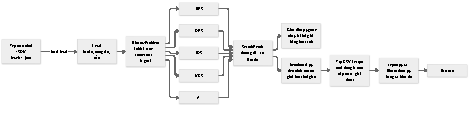
\includegraphics[width=\linewidth,height=0.78\textheight,keepaspectratio]{images/sodo1.pdf}
\end{sodo}

\subsection{Giao diện đồ hoạ}

\begin{itemize}
\item \textbf{Điều khiển:} phím mũi tên hoặc W/A/S/D để lăn khối; phím Space để đổi khối được điều khiển khi đang tách; phím R để chơi lại màn.
\item \textbf{Nút bấm:} \texttt{\textless{} Prev} / \texttt{Next \textgreater{}} (chọn màn), \texttt{New Game}, \texttt{Restart}, và bốn nút \texttt{Solve BFS}, \texttt{Solve DFS}, \texttt{Solve UCS}, \texttt{Solve A*}.
\item \textbf{Chạy solver:} thuật toán chạy trên một luồng riêng nên giao diện không bị treo. Khi có kết quả, lời giải được phát lại bằng hoạt ảnh lăn khối, và bảng \emph{Solver Metrics} hiển thị tên thuật toán, độ dài lời giải, số nút mở rộng, thời gian tìm kiếm và cost của lời giải.
\end{itemize}

\section{Hình thức hoá bài toán tìm kiếm}

Mục này mô tả bài toán theo đúng các thành phần của một bài toán tìm kiếm: trạng thái, hành động, mô hình chuyển trạng thái, kiểm tra đích, hàm chi phí và heuristic. Mục cuối trình bày cách các thuật toán tránh duyệt lại trạng thái. Toàn bộ mô hình nằm trong \texttt{bloxorz/core} và được mọi thuật toán dùng chung.

\subsection{Màn chơi và định dạng tệp}

Một màn chơi là một lưới ký tự trong tệp JSON, kèm danh sách công tắc. Toạ độ ghi dạng \texttt{[hàng, cột]}, bắt đầu từ 0, hàng 0 ở trên cùng.

{\renewcommand{\arraystretch}{1.25}
\begin{longtable}{|l|l|l|}
\hline
\textbf{Ký tự} & \textbf{Ô} & \textbf{Ghi chú} \\ \hline
\endhead
\hline
\endlastfoot
\texttt{.} & Ô trống (void) & Không có sàn \\ \hline
\texttt{\#} & Sàn &  \\ \hline
\texttt{S} & Sàn, vị trí bắt đầu & Đúng 1 ô; khối bắt đầu ở tư thế đứng \\ \hline
\texttt{G} & Lỗ đích & Đúng 1 ô \\ \hline
\texttt{F} & Ô dễ vỡ &  \\ \hline
\texttt{-} / \texttt{=} & Cầu, đóng / mở lúc đầu &  \\ \hline
\texttt{O} & Công tắc mềm & Cần một mục trong \texttt{switches} \\ \hline
\texttt{X} & Công tắc nặng & Cần một mục trong \texttt{switches} \\ \hline
\texttt{T} & Công tắc tách & Cần một mục trong \texttt{switches} \\
\end{longtable}
}

\begin{Verbatim}[breaklines=true, fontsize=\footnotesize, frame=single]
{
  "name": "Ví dụ",
  "grid": ["S#O-=#", "##X--#", "#T#FFG"],
  "switches": [
    {"pos": [0, 2], "effect": "toggle", "bridges": [[0, 3], [0, 4]]},
    {"pos": [1, 2], "effect": "open",   "bridges": [[1, 3], [1, 4]]},
    {"pos": [2, 1], "targets": [[0, 0], [2, 0]]}
  ]
}
\end{Verbatim}

\begin{itemize}
\item Công tắc mềm và công tắc nặng có \texttt{effect} (\texttt{toggle}: đảo trạng thái, \texttt{open}: mở, \texttt{close}: đóng) và \texttt{bridges} (các ô cầu mà công tắc điều khiển).
\item Công tắc tách có \texttt{targets}: hai ô nơi hai khối lập phương xuất hiện. Hai ô này phải khác nhau, không phải ô trống và không kề cạnh nhau, vì hai khối kề nhau sẽ ghép lại ngay (mục 3.4.3).
\item Bộ đọc màn kiểm tra toàn bộ các ràng buộc trên. Tệp sai định dạng bị từ chối với thông báo lỗi chỉ rõ vị trí.
\end{itemize}

\begin{figure}[!htbp]
\centering
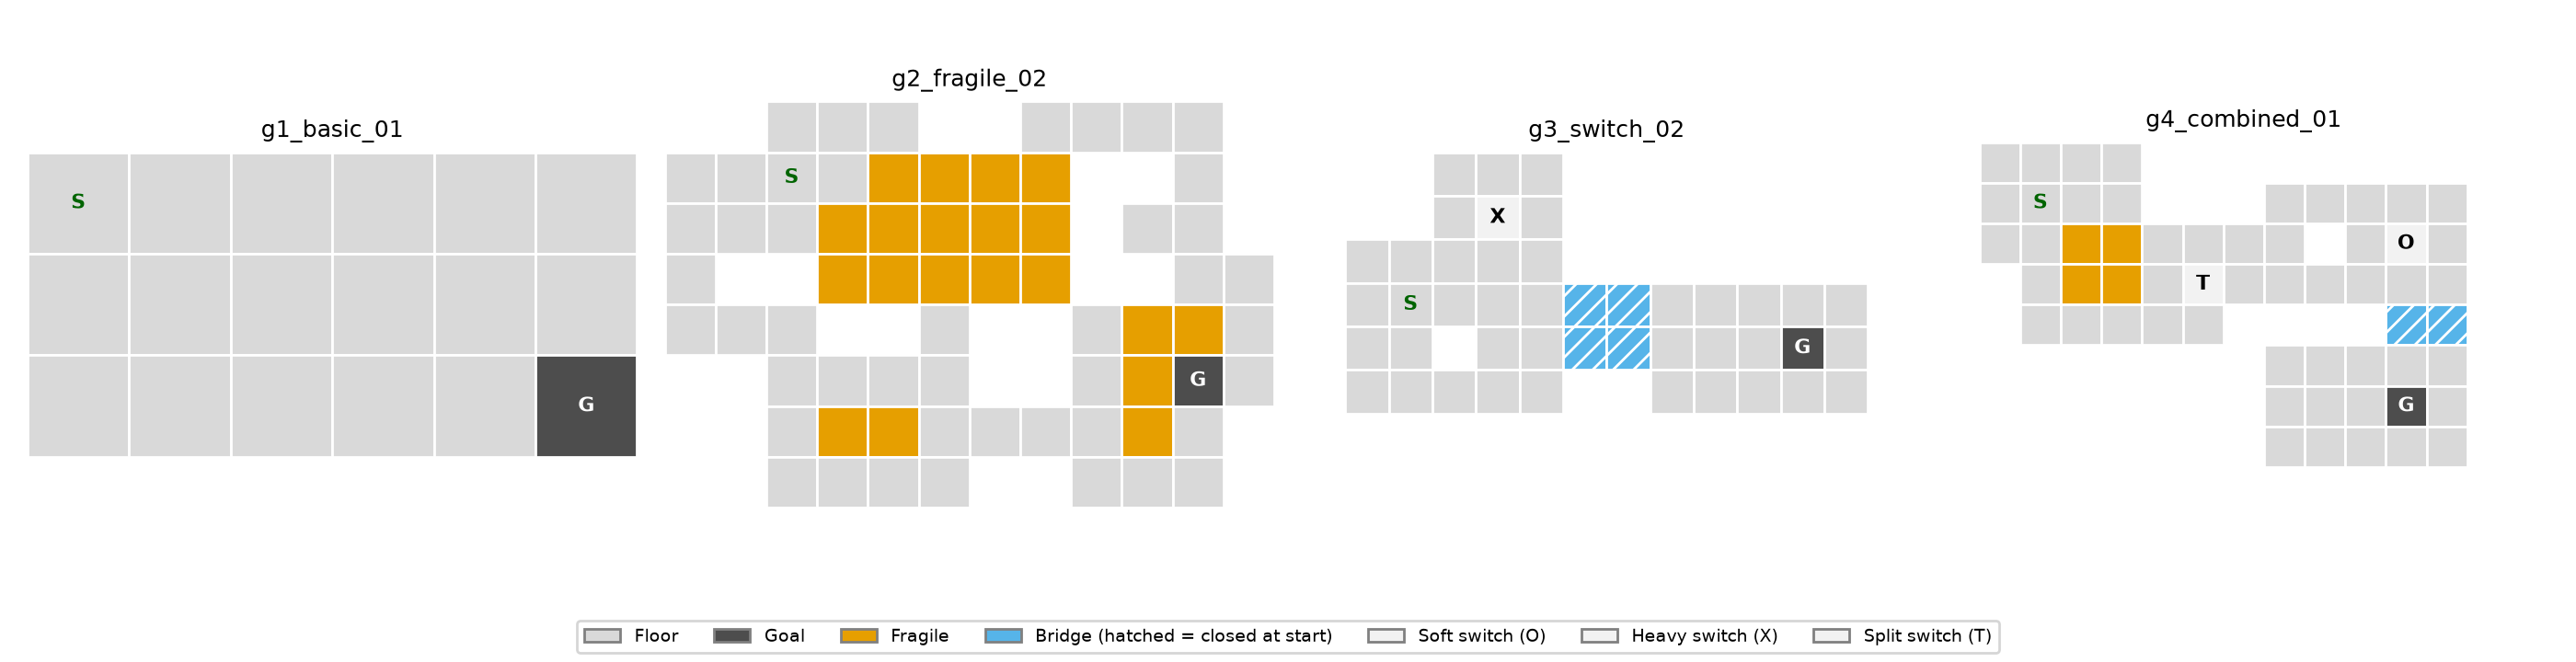
\includegraphics[width=\linewidth,height=0.45\textheight,keepaspectratio]{images/fig_level_groups.png}
\caption{Bốn màn đại diện cho bốn nhóm độ khó (g1: cơ bản; g2: ô dễ vỡ; g3: công tắc và cầu; g4: kết hợp). Ký hiệu S là ô xuất phát, G là ô đích. Các ô cầu gạch chéo ở trạng thái đóng khi bắt đầu.}
\end{figure}

\subsection{Biểu diễn trạng thái}

Phần tĩnh của màn chơi (lưới ô, danh sách công tắc, vị trí đích) nằm trong đối tượng \texttt{Level}. Đối tượng này bất biến và được mọi nút tìm kiếm dùng chung, nên không thuộc trạng thái. Trạng thái chỉ chứa phần thay đổi được, là một \texttt{NamedTuple} \textbf{bất biến và băm được}:

\[s = \langle \text{block}, \text{cubes}, \text{bridges} \rangle\]

{\renewcommand{\arraystretch}{1.25}
\begin{longtable}{|>{\raggedright\arraybackslash}p{0.143\linewidth}|>{\raggedright\arraybackslash}p{0.787\linewidth}|}
\hline
\textbf{Thành phần} & \textbf{Ý nghĩa} \\ \hline
\endhead
\hline
\endlastfoot
\texttt{block} & Khi khối còn nguyên: \texttt{Block(row, col, orientation)} với tư thế \texttt{STANDING}, \texttt{HORIZONTAL} hoặc \texttt{VERTICAL}. Bằng \texttt{None} khi khối đã tách. \\ \hline
\texttt{cubes} & Khi đã tách: \texttt{((r₁, c₁), (r₂, c₂))}, \textbf{phần tử đầu là khối đang được điều khiển}. Bằng \texttt{None} khi khối còn nguyên. \\ \hline
\texttt{bridges} & Số nguyên dùng làm mặt nạ bit: bit thứ \emph{i} bằng 1 nghĩa là ô cầu thứ \emph{i} đang mở. \\
\end{longtable}
}

\begin{itemize}
\item \textbf{Ô neo.} \texttt{Block} được neo ở ô trên cùng bên trái. Tư thế đứng chiếm ô (r, c); nằm ngang chiếm (r, c) và (r, c+1); nằm dọc chiếm (r, c) và (r+1, c).
\item \textbf{Cấu hình cầu thuộc trạng thái.} Hai trạng thái có cùng vị trí khối nhưng khác trạng thái đóng/mở của cầu là \textbf{hai trạng thái khác nhau}, vì khả năng đi tiếp của chúng khác nhau. Đề yêu cầu điều này (mục 3.1 của đề).
\item \textbf{Khối đang điều khiển thuộc trạng thái.} Khi đã tách, \texttt{((a, b), (b, a))} hoán vị là hai trạng thái khác nhau, vì nước đi tiếp theo di chuyển khối khác nhau.
\item \textbf{Mặt nạ bit thay cho tập hợp.} Một số nguyên vừa gọn bộ nhớ, vừa cho phép đóng, mở hay đảo nhiều cầu cùng lúc bằng một phép toán bit (mục 3.4.3).
\end{itemize}

\textbf{Kích thước không gian trạng thái.} Với lưới R×C và m ô cầu, số trạng thái nhiều nhất là 3·R·C·2$^{m}$ (khối nguyên) cộng (R·C)²·2$^{m}$ (khối đã tách). Không gian hữu hạn là cơ sở để chứng minh các thuật toán ở mục 4 và 5 luôn dừng. Trong thực tế số trạng thái đạt tới được nhỏ hơn nhiều: màn lớn nhất (\texttt{g4\_\allowbreak{}combined\_\allowbreak{}04}) có 13 889 trạng thái đạt tới được.

\subsection{Hành động}

Tập hành động là \textbf{Lên (U), Xuống (D), Trái (L), Phải (R)}, cộng thêm \textbf{đổi khối (S)} khi khối đang tách. Các hành động luôn được liệt kê theo \textbf{thứ tự cố định U, D, L, R, (S)}, nên mọi lần chạy cho cùng một kết quả và các thí nghiệm tái lập được. Mỗi trạng thái vì vậy có tối đa 4 nước đi khi khối còn nguyên và tối đa 5 khi đã tách.

\subsection{Mô hình chuyển trạng thái}

Hàm \texttt{result(s, a)} trả về trạng thái kế tiếp, hoặc \texttt{None} nếu nước đi làm khối rơi. Hàm thực hiện bốn bước:

\begin{enumerate}
\item Nếu \texttt{a} là đổi khối S: hoán đổi hai phần tử của \texttt{cubes} và trả về ngay. Vị trí không đổi nên không ô nào phản ứng.
\item Tính vị trí mới: khối nguyên lăn theo bảng chuyển tư thế (mục 3.4.1); khối đã tách thì chỉ khối đang điều khiển đi một ô.
\item Kiểm tra vị trí mới có hợp lệ không (mục 3.4.2). Nếu không, trả về \texttt{None}.
\item Áp dụng hiệu ứng của các ô dưới khối (mục 3.4.3). Bước này có thể đổi cấu hình cầu, tách khối, ghép khối, hoặc làm khối rơi.
\end{enumerate}

\subsubsection{Bảng chuyển tư thế}

Mỗi cặp (tư thế, hướng) ánh xạ xác định tới một cặp (tư thế mới, ô neo mới):

{\small\renewcommand{\arraystretch}{1.25}
\begin{longtable}{|l|l|l|l|l|}
\hline
\textbf{Tư thế \textbackslash{} Hướng} & \textbf{Lên} & \textbf{Xuống} & \textbf{Trái} & \textbf{Phải} \\ \hline
\endhead
\hline
\endlastfoot
Đứng (r, c) & Dọc (r−2, c) & Dọc (r+1, c) & Ngang (r, c−2) & Ngang (r, c+1) \\ \hline
Ngang (r, c) & Ngang (r−1, c) & Ngang (r+1, c) & Đứng (r, c−1) & Đứng (r, c+2) \\ \hline
Dọc (r, c) & Đứng (r−1, c) & Đứng (r+2, c) & Dọc (r, c−1) & Dọc (r, c+1) \\
\end{longtable}
}

\begin{sodo}[!htbp]
\centering
\caption{Chuyển tư thế của khối khi lăn}
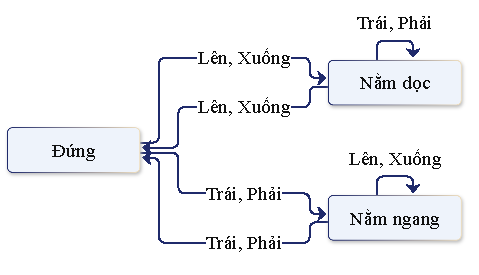
\includegraphics[width=0.62\linewidth,height=0.3\textheight,keepaspectratio]{images/sodo2.pdf}
\end{sodo}

Khối đứng lăn thì ngã thành nằm theo hướng lăn; khối nằm lăn dọc theo trục dài thì dựng lên đứng; khối nằm lăn ngang qua trục dài thì vẫn nằm. Cả 12 ô của bảng đều có test riêng.

\subsubsection{Tính hợp lệ của nước đi}

Một vị trí là hợp lệ khi thoả \textbf{mọi} điều kiện sau:

\begin{itemize}
\item mọi ô khối chiếm đều nằm trong lưới, không phải ô trống và không phải cầu đang đóng (cầu đóng được coi như ô trống);
\item khối nguyên \textbf{đang đứng} thì không nằm trên ô dễ vỡ (toàn bộ trọng lượng dồn vào một ô làm ô vỡ);
\item khi đã tách, hai khối lập phương không trùng ô.
\end{itemize}

Khối nằm (trọng lượng chia cho hai ô) và khối lập phương đơn (nửa trọng lượng) được phép nằm trên ô dễ vỡ.

\subsubsection{Hiệu ứng của ô đặc biệt}

Sau một nước đi hợp lệ, các công tắc dưới khối được kích hoạt theo quy tắc:

{\renewcommand{\arraystretch}{1.25}
\begin{longtable}{|>{\raggedright\arraybackslash}p{0.095\linewidth}|>{\raggedright\arraybackslash}p{0.400\linewidth}|>{\raggedright\arraybackslash}p{0.400\linewidth}|}
\hline
\textbf{Loại công tắc} & \textbf{Điều kiện kích hoạt} & \textbf{Hiệu ứng} \\ \hline
\endhead
\hline
\endlastfoot
Mềm (\texttt{O}) & Bất kỳ phần nào của khối đè lên: đứng, nằm, hoặc một khối lập phương & Đóng, mở hoặc đảo các cầu liên kết \\ \hline
Nặng (\texttt{X}) & Chỉ khối nguyên đứng thẳng trên ô & Đóng, mở hoặc đảo các cầu liên kết \\ \hline
Tách (\texttt{T}) & Chỉ khối nguyên đứng thẳng trên ô & Khối biến mất, hai khối lập phương xuất hiện tại \texttt{targets}; khối tại \texttt{targets[0]} được điều khiển trước \\
\end{longtable}
}

\begin{itemize}
\item \textbf{Cập nhật cầu bằng phép toán bit.} Mỗi công tắc lưu sẵn một mặt nạ M gồm các bit của những cầu nó điều khiển. Đảo trạng thái là \texttt{B \textasciicircum{} M}, mở là \texttt{B \textbar{} M}, đóng là \texttt{B \& \textasciitilde{}M}, với B là \texttt{bridges}.
\item \textbf{Cầu đóng dưới chân khối.} Nếu một công tắc đóng đúng cây cầu khối đang nằm lên, khối mất chỗ đỡ và rơi: nước đi trả về \texttt{None}.
\item \textbf{Chế độ tách.} Mỗi nước đi chỉ di chuyển khối đang điều khiển, một ô một lần. Khối lập phương không kích hoạt được công tắc nặng hay công tắc tách, và không thắng được khi đứng trên đích. Khi đang tách, \textbf{chỉ khối vừa di chuyển} mới kích hoạt công tắc dưới chân nó. Khối đứng yên không kích hoạt lại công tắc nó đang đứng.
\item \textbf{Ghép khối.} Sau mỗi nước đi của một khối lập phương, nếu hai khối kề cạnh nhau (khoảng cách Manhattan bằng 1) thì chúng \textbf{tự ghép ngay} thành một khối nằm: cùng hàng thì thành khối nằm ngang, cùng cột thì thành khối nằm dọc. Hai khối kề chéo không ghép. Vì ghép xảy ra ngay khi vừa kề nhau, ngay trước mọi bước ghép hai khối luôn cách nhau 2 ô.
\end{itemize}

\subsubsection{Các trường hợp biên đã thống nhất}

Đề không quy định một số tình huống. Nhóm thống nhất cách xử lý như sau:

{\renewcommand{\arraystretch}{1.25}
\begin{longtable}{|>{\centering\arraybackslash}p{0.068\linewidth}|>{\raggedright\arraybackslash}p{0.414\linewidth}|>{\raggedright\arraybackslash}p{0.414\linewidth}|}
\hline
\textbf{Mã} & \textbf{Tình huống} & \textbf{Cách xử lý} \\ \hline
\endhead
\hline
\endlastfoot
EC-01 & Công tắc đóng chính cây cầu khối đang nằm lên & Khối mất chỗ đỡ, rơi xuống (thua) \\ \hline
EC-02 & Khối lập phương đứng yên trên công tắc khi khối kia di chuyển & Không kích hoạt lại công tắc dưới khối đứng yên \\ \hline
EC-03 & Hành động đổi khối S & Không di chuyển, không kích hoạt công tắc, giữ nguyên cầu \\ \hline
EC-04 & Ghép khối khi một khối đang đứng trên công tắc mềm & Công tắc không bị kích hoạt lại, vì khối đó không di chuyển \\ \hline
EC-05 & Hai khối lập phương đi vào cùng một ô & Nước đi không hợp lệ (thực tế không xảy ra, vì hai khối đã ghép từ khi kề nhau) \\ \hline
EC-06 & Một trong hai khối lập phương rơi & Thua ngay \\ \hline
EC-07 & Khối nằm đè cùng lúc lên hai công tắc mềm & Kích hoạt lần lượt cả hai; nếu cùng đảo một cầu thì cầu đảo hai lần \\ \hline
EC-08 & Ghép khối ngay trên ô dễ vỡ & An toàn, vì khối sau khi ghép luôn ở tư thế nằm \\ \hline
EC-09 & Vị trí xuất hiện sau khi tách là một công tắc mềm & Công tắc mềm đó được kích hoạt ngay \\ \hline
EC-10 & Vị trí xuất hiện sau khi tách là ô trống hoặc cầu đóng & Khối lập phương rơi (thua) \\
\end{longtable}
}

\subsubsection{Sinh trạng thái kế tiếp}

Hàm \texttt{successors(s)} áp dụng \texttt{result} cho từng hành động theo thứ tự cố định và bỏ các nước đi làm khối rơi (Sơ đồ 3).

\begin{sodo}[!htbp]
\centering
\caption{Sinh các trạng thái kế tiếp \texttt{successors(s)}}
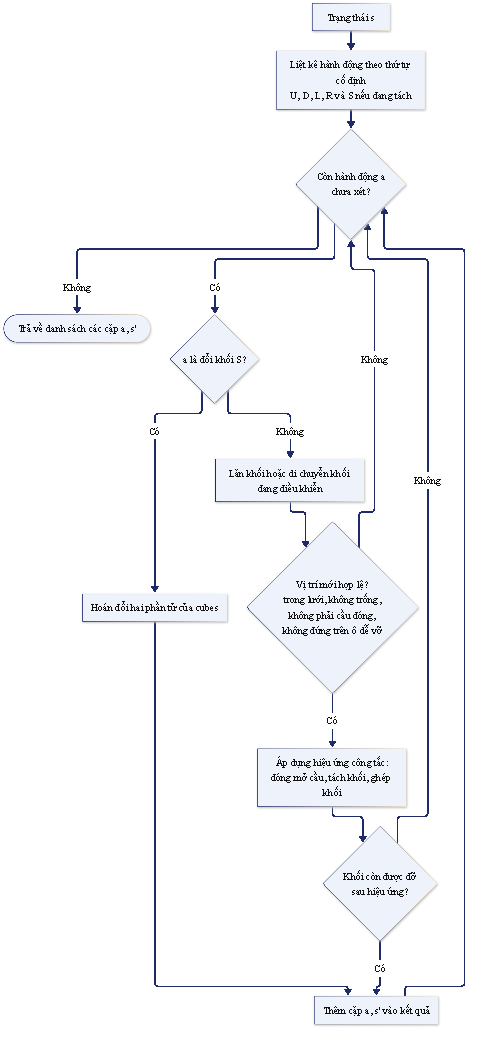
\includegraphics[width=0.95\linewidth,height=0.78\textheight,keepaspectratio]{images/sodo3.pdf}
\end{sodo}

\subsection{Kiểm tra đích}

\texttt{is\_\allowbreak{}goal(s)} đúng khi và chỉ khi khối \textbf{còn nguyên}, ở tư thế \textbf{đứng}, và nằm trên ô đích. Khối nằm vắt qua ô đích hay một khối lập phương đơn trên ô đích đều không thắng.

\subsection{Hàm chi phí}

Nhóm dùng hai hàm chi phí, cùng có dạng \texttt{cost(s, a, s')}:

{\renewcommand{\arraystretch}{1.25}
\begin{longtable}{|>{\raggedright\arraybackslash}p{0.102\linewidth}|>{\raggedright\arraybackslash}p{0.469\linewidth}|>{\raggedright\arraybackslash}p{0.324\linewidth}|}
\hline
\textbf{Hàm} & \textbf{Định nghĩa} & \textbf{Dùng cho} \\ \hline
\endhead
\hline
\endlastfoot
\texttt{unit\_\allowbreak{}cost} & Mọi nước đi tốn 1 & BFS, DFS, IDS (tối ưu theo số nước đi) \\ \hline
\texttt{physics\_\allowbreak{}cost} & Nước đi kết thúc ở tư thế đứng tốn 3, mọi nước đi khác tốn 1 & UCS, A* \\
\end{longtable}
}

\texttt{physics\_\allowbreak{}cost} dựa trên độ nâng trọng tâm của khối khi lăn: dựng khối từ nằm lên đứng phải nâng trọng tâm cao gấp khoảng 3 lần so với một bước lăn ngang. Phần xây dựng và lý giải chi tiết ở mục 5.1.4. Chi phí nhỏ nhất của một bước là 1 với cả hai hàm; heuristic của A* dựa vào tính chất này (mục 5.3).

\subsection{Heuristic}

A* dùng một heuristic ước lượng chi phí còn lại từ khoảng cách Manhattan đến đích chia 2 (một bước lăn đi tối đa 2 ô), xét thêm đường đi qua công tắc tách, và không bao giờ nhỏ hơn chi phí của bước dựng đứng cuối cùng. Công thức và chứng minh tính chấp nhận được, tính nhất quán đối với chính hàm chi phí đã chọn được trình bày ở mục 5.3.

\subsection{Tránh duyệt lại trạng thái}

Do khối có thể lăn qua lại, từ một trạng thái có thể quay về chính nó sau vài nước đi (chẳng hạn lăn sang phải rồi lăn lại sang trái). Đồ thị trạng thái vì vậy có \textbf{chu trình}, và nhiều đường đi khác nhau dẫn tới cùng một trạng thái. Nếu duyệt như duyệt cây, DFS có thể lặp vô hạn còn BFS lãng phí thời gian vào các nhánh trùng lặp. Cả năm thuật toán đều là \textbf{tìm kiếm trên đồ thị}: trạng thái băm được nên dùng trực tiếp làm khoá của \texttt{dict} hoặc phần tử của \texttt{set}, kiểm tra ``đã gặp'' trong thời gian O(1).

{\renewcommand{\arraystretch}{1.25}
\begin{longtable}{|>{\raggedright\arraybackslash}p{0.082\linewidth}|>{\raggedright\arraybackslash}p{0.361\linewidth}|>{\raggedright\arraybackslash}p{0.452\linewidth}|}
\hline
\textbf{Thuật toán} & \textbf{Cấu trúc chống lặp} & \textbf{Quy tắc} \\ \hline
\endhead
\hline
\endlastfoot
BFS & \texttt{parent} (dict) & Trạng thái đã có trong \texttt{parent} thì bỏ qua; mỗi trạng thái vào hàng đợi tối đa một lần \\ \hline
DFS & \texttt{visited} (set) & Đánh dấu khi đưa vào ngăn xếp; mỗi trạng thái vào ngăn xếp tối đa một lần \\ \hline
IDS & \texttt{reached} (dict: trạng thái → độ sâu nhỏ nhất) & Trong mỗi lượt, chỉ đưa lại vào ngăn xếp khi gặp ở độ sâu nhỏ hơn \\ \hline
UCS & \texttt{best\_\allowbreak{}cost} (dict) & Chỉ đẩy vào hàng đợi khi tìm được chi phí nhỏ hơn; bản sao cũ bị bỏ qua khi lấy ra \\ \hline
A* & \texttt{best\_\allowbreak{}g} (dict) & Như UCS; heuristic nhất quán nên mỗi trạng thái được mở rộng tối đa một lần \\
\end{longtable}
}

\subsection{Kiểm thử mô hình}

Mô hình bài toán được kiểm thử tự động bằng \texttt{pytest} (212 test cho toàn bộ dự án):

\begin{itemize}
\item \textbf{Bảng chuyển tư thế:} đủ 12 cặp (tư thế, hướng), và kiểm tra lăn ngược thì về vị trí cũ.
\item \textbf{Bộ đọc màn:} các màn hợp lệ, và từng trường hợp tệp sai định dạng.
\item \textbf{Giao diện bài toán:} rơi khỏi bàn, rơi vào ô trống, thắng và không thắng, thứ tự hành động, đổi khối, phát lại lời giải. Trên màn 1 của trò chơi gốc, lời giải tối ưu 7 nước \texttt{RDDRRDR} đưa khối vào đích, và BFS tìm đúng lời giải này.
\item \textbf{Luật ô đặc biệt (29 test):} ô dễ vỡ và cầu; công tắc mềm và nặng; đóng, mở, đảo cầu và cầu sập dưới chân; công tắc tách; ghép khối; va chạm giữa hai khối lập phương; và một màn có đủ chu trình tách, đổi khối, ghép lại, về đích được BFS giải đúng.
\end{itemize}

\section{Các thuật toán tìm kiếm không có thông tin: BFS, DFS, IDS}

Ba thuật toán trong mục này không dùng heuristic ước lượng khoảng cách đến đích, và đều coi mỗi nước đi có chi phí 1. Đề cho phép dùng IDS thay cho DFS; nhóm cài đặt \textbf{cả hai} và đưa cả hai vào thực nghiệm. Cả ba được cài đặt bằng tay, chỉ dùng các cấu trúc dữ liệu chuẩn của Python (\texttt{collections.deque}, \texttt{list}, \texttt{dict}, \texttt{set}).

\subsection{Khung tìm kiếm trên đồ thị dùng chung}

Ba thuật toán cùng một khung; chúng chỉ khác nhau ở \textbf{cấu trúc dữ liệu của frontier} (tập các nút đã sinh nhưng chưa mở rộng) và \textbf{cách chọn nút để mở rộng tiếp theo}:

\begin{Verbatim}[breaklines=true, fontsize=\footnotesize, frame=single]
GRAPH-SEARCH(problem):
    frontier <- { s0 }                  # s0 = problem.initial_state
    reached  <- { s0 }                  # các trạng thái đã gặp, kèm con trỏ cha
    trong khi frontier không rỗng:
        s <- CHỌN-VÀ-LẤY-RA(frontier)   # điểm khác nhau giữa các thuật toán
        nếu s là đích: dựng lại đường đi bằng cách lần ngược theo con trỏ cha
        mở rộng s: với mỗi (a, s') trong successors(s):
            nếu s' chưa có trong reached:
                ghi nhận s' (cha = s, hành động = a), đưa s' vào frontier
    trả về thất bại
\end{Verbatim}

Khung trên kiểm tra đích lúc lấy nút ra, nên nút đích không bao giờ bị mở rộng. DFS và IDS dùng đúng cách này; BFS kiểm tra sớm hơn, ngay khi nút được sinh ra (mục 4.2.3).

{\renewcommand{\arraystretch}{1.25}
\begin{longtable}{|>{\raggedright\arraybackslash}p{0.083\linewidth}|>{\raggedright\arraybackslash}p{0.306\linewidth}|>{\raggedright\arraybackslash}p{0.182\linewidth}|>{\raggedright\arraybackslash}p{0.289\linewidth}|}
\hline
\textbf{Thuật toán} & \textbf{Frontier} & \textbf{Chọn nút} & \textbf{Ý nghĩa} \\ \hline
\endhead
\hline
\endlastfoot
BFS & Hàng đợi FIFO (\texttt{deque}) & Nút vào sớm nhất & Duyệt theo từng lớp độ sâu \\ \hline
DFS & Ngăn xếp LIFO (\texttt{list}) & Nút vào muộn nhất & Đi sâu trước, quay lui sau \\ \hline
IDS & Ngăn xếp, có giới hạn độ sâu tăng dần & Như DFS trong mỗi lượt & Lặp lại DFS với giới hạn 1, 2, 3, … \\
\end{longtable}
}

\textbf{Ghi nhận đường đi.} Thay vì lưu kèm danh sách hành động trong mỗi phần tử của frontier (tốn thêm bộ nhớ tỉ lệ với độ sâu cho mỗi nút), mỗi trạng thái chỉ lưu \texttt{(trạng thái cha, hành động đã dùng)} trong từ điển \texttt{parent}. Khi tìm thấy đích, đường đi được dựng bằng cách lần ngược từ đích về trạng thái đầu rồi đảo thứ tự.

\textbf{Quy ước đếm số nút mở rộng (expanded nodes).} Một nút được tính là \emph{đã mở rộng} khi nó được lấy ra khỏi frontier \textbf{và} các nút con của nó được sinh ra (gọi \texttt{successors}). Nút đích không được tính vì không cần sinh nút con của nó. Quy ước này được áp dụng thống nhất cho mọi thuật toán thông qua \texttt{MetricsTracker.count\_\allowbreak{}expansion()}, nhờ vậy các con số có thể so sánh với nhau. Với IDS, số này là tổng cộng dồn qua tất cả các lượt lặp.

\subsection{Tìm kiếm theo chiều rộng (BFS)}

\subsubsection{Ý tưởng}

BFS mở rộng toàn bộ các trạng thái cách trạng thái đầu 0 nước đi, rồi đến 1 nước, 2 nước, … Mọi trạng thái ở độ sâu k đều được mở rộng trước mọi trạng thái ở độ sâu k+1. Frontier là hàng đợi FIFO, cài đặt bằng \texttt{collections.deque} để cả \texttt{append} (thêm vào cuối) lẫn \texttt{popleft} (lấy từ đầu) đều có chi phí O(1).

\subsubsection{Mã giả}

\begin{Verbatim}[breaklines=true, fontsize=\footnotesize, frame=single]
BFS(problem):
    s0 <- problem.initial_state
    nếu is_goal(s0): trả về []                       # 0 nước đi, 0 nút mở rộng
    frontier <- deque([s0])
    parent   <- { s0: None }                           # đồng thời là tập các trạng thái đã thăm
    trong khi frontier không rỗng:
        s <- frontier.popleft()
        expanded <- expanded + 1
        với mỗi (a, s') trong successors(s):          # thứ tự U, D, L, R (S nếu đang tách)
            nếu s' chưa có trong parent:
                parent[s'] <- (s, a)
                nếu is_goal(s'): trả về reconstruct(parent, s')   # kiểm tra đích sớm
                frontier.append(s')
    trả về None
\end{Verbatim}

\subsubsection{Các quyết định cài đặt}

\begin{itemize}
\item \textbf{Kiểm tra đích sớm.} Đích được kiểm tra ngay khi trạng thái được \emph{sinh ra}, không đợi đến khi nó được lấy khỏi hàng đợi. Điều này đúng vì mọi nước đi có cùng chi phí nên trạng thái đích được sinh ra đầu tiên chắc chắn nằm ở độ sâu nhỏ nhất. Cách làm này tránh việc phải mở rộng thêm cả một lớp độ sâu trước khi trả về (Russell và Norvig, AIMA). Hệ quả là nút đích ở độ sâu d được phát hiện khi mở rộng một nút ở độ sâu d−1, và Hình 2 cho thấy lớp cuối cùng được mở rộng chỉ có độ sâu d−1.
\item \textbf{Từ điển \texttt{parent} đóng hai vai trò}: lưu con trỏ cha để dựng đường đi và là tập đã thăm để chống lặp. Một trạng thái chỉ vào frontier khi chưa từng xuất hiện trong \texttt{parent}, do đó mỗi trạng thái được mở rộng tối đa một lần.
\item \textbf{Frontier chỉ chứa trạng thái}, không chứa đường đi, như đã nêu ở mục 4.1.
\end{itemize}

\subsubsection{Ví dụ chạy tay trên màn g1\_basic\_01}

Màn gồm lưới 3 hàng × 6 cột toàn sàn thường, xuất phát tại (0,0), đích tại (2,5). Kí hiệu trạng thái: chữ cái là tư thế (S: đứng, H: nằm ngang, V: nằm dọc) kèm ô neo (hàng, cột).

{\renewcommand{\arraystretch}{1.25}
\begin{longtable}{|>{\raggedleft\arraybackslash}p{0.073\linewidth}|>{\raggedright\arraybackslash}p{0.122\linewidth}|>{\raggedright\arraybackslash}p{0.349\linewidth}|>{\raggedright\arraybackslash}p{0.316\linewidth}|}
\hline
\textbf{Bước} & \textbf{Nút được lấy ra} & \textbf{Các nút con sinh ra (hành động: trạng thái)} & \textbf{Ghi chú} \\ \hline
\endhead
\hline
\endlastfoot
1 & S(0,0) & D: V(1,0); R: H(0,1) & U và L ra ngoài lưới nên bị loại \\ \hline
2 & V(1,0) & U: S(0,0); R: V(1,1) & S(0,0) đã có trong \texttt{parent} nên bị bỏ qua \\ \hline
3 & H(0,1) & D: H(1,1); L: S(0,0); R: S(0,3) & S(0,0) bị bỏ qua \\ \hline
4 & V(1,1) & U: S(0,1); L: V(1,0); R: V(1,2) & V(1,0) bị bỏ qua \\
\end{longtable}
}

Số nút được mở rộng theo từng độ sâu là \texttt{[1, 2, 3, 7, 6, 8, 9, 5]} (tổng 41 nút). Nút đích được sinh ra ở độ sâu 8 khi đang mở rộng một nút ở độ sâu 7, và đường đi trả về là \textbf{DRRURDDR} (8 nước đi).

\subsubsection{Tính chất và chứng minh}

\textbf{Tính dừng và tính đầy đủ.} Không gian trạng thái hữu hạn (mục 3.2) và mỗi trạng thái vào frontier tối đa một lần, nên vòng lặp luôn kết thúc. Nếu đích đạt tới được thì nó sẽ được sinh ra ở một lúc nào đó, vì mọi trạng thái đạt tới được đều lần lượt được mở rộng. Nếu frontier cạn mà chưa gặp đích, màn không có lời giải. Do đó BFS đầy đủ và quyết định được tính giải được của màn.

\textbf{Tính tối ưu theo số nước đi.} Chứng minh bằng quy nạp theo độ sâu k: \emph{mọi trạng thái ở độ sâu k (khoảng cách ngắn nhất tính bằng số nước đi từ trạng thái đầu) được đưa vào hàng đợi trước mọi trạng thái ở độ sâu k+1, và \texttt{parent} của nó lưu đúng một đường đi có độ dài k.}

\begin{itemize}
\item Cơ sở: độ sâu 0 chỉ có s0.
\item Bước quy nạp: mọi trạng thái ở độ sâu k+1 có một nút cha ở độ sâu k. Theo giả thiết, các nút ở độ sâu k đều được lấy ra (và mở rộng) trước các nút ở độ sâu k+1, nên trạng thái ở độ sâu k+1 được sinh ra đầu tiên từ một nút độ sâu k. Không nút nào ở độ sâu lớn hơn có thể sinh ra nó sớm hơn vì chúng được lấy ra sau.
\end{itemize}

Do đó lần đầu một trạng thái được phát hiện chính là lúc nó được phát hiện bằng đường ngắn nhất, và đích được phát hiện lần đầu cho lời giải có số nước đi nhỏ nhất. Tính chất này chỉ đảm bảo tối ưu theo \textbf{số nước đi}; không đảm bảo tối ưu theo \texttt{physics\_\allowbreak{}cost} (mục 6.5).

\textbf{Độ phức tạp.} Mỗi trạng thái được mở rộng tối đa một lần, mỗi lần sinh tối đa b nút con (b ≤ 4, hoặc 5 khi đang tách) và mỗi thao tác tra bảng băm là O(1). Thời gian là O(b·\textbar{}S\textbar{}) = O(\textbar{}S\textbar{}), và theo độ sâu lời giải d còn bị chặn bởi O(b$^{d}$). Bộ nhớ là O(\textbar{}S\textbar{}) vì phải giữ cả frontier lẫn \texttt{parent}. Thực tế số nút theo từng độ sâu tăng chậm hơn nhiều so với b$^{d}$ vì đồ thị trạng thái có nhiều đường song song và chu trình (Hình 2).

\begin{figure}[!htbp]
\centering
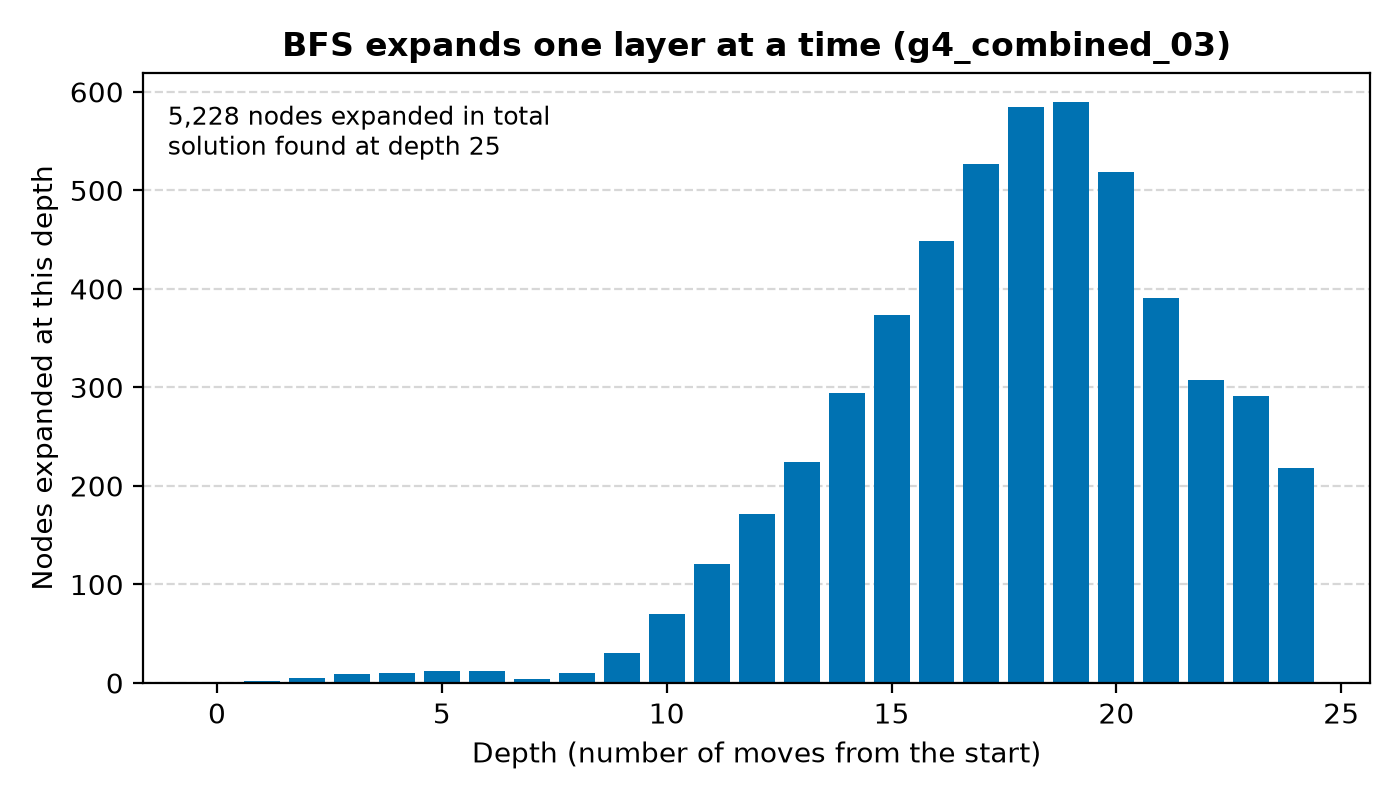
\includegraphics[width=\linewidth,height=0.45\textheight,keepaspectratio]{images/fig_bfs_layers.png}
\caption{Số nút BFS mở rộng ở từng độ sâu trên màn g4\_combined\_03: tổng 5.228 nút, lời giải ở độ sâu 25. Số nút theo lớp tăng đến cực đại ở độ sâu 18–19 rồi giảm.}
\end{figure}

\subsection{Tìm kiếm theo chiều sâu (DFS)}

\subsubsection{Ý tưởng}

DFS luôn đi sâu theo một nhánh cho đến khi gặp ngõ cụt (mọi nước đi đều dẫn đến trạng thái đã thăm hoặc không hợp lệ), rồi quay lui để thử nhánh khác. Frontier là ngăn xếp LIFO. Thuật toán được cài đặt \textbf{bằng ngăn xếp tường minh} (một \texttt{list} với \texttt{append} và \texttt{pop}) mà không dùng đệ quy, để không gặp \texttt{RecursionError} khi lời giải dài (DFS tìm được lời giải 304 nước ở màn g4\_combined\_02).

\subsubsection{Mã giả}

\begin{Verbatim}[breaklines=true, fontsize=\footnotesize, frame=single]
DFS(problem, max_depth = None):
    s0 <- problem.initial_state
    nếu is_goal(s0): trả về []
    stack   <- [(s0, 0)]
    parent  <- { s0: None };  visited <- { s0 }
    trong khi stack không rỗng:
        (s, depth) <- stack.pop()
        nếu is_goal(s): trả về reconstruct(parent, s)
        nếu max_depth != None và depth >= max_depth: tiếp tục vòng lặp       # cắt nhánh
        expanded <- expanded + 1
        với mỗi (a, s') trong reversed(successors(s)):
            nếu s' chưa có trong visited:
                visited.add(s');  parent[s'] <- (s, a)
                stack.append((s', depth + 1))
    trả về None
\end{Verbatim}

\subsubsection{Các quyết định cài đặt}

\begin{itemize}
\item \textbf{Duyệt \texttt{reversed(successors(s))}.} Ngăn xếp lấy phần tử \emph{đưa vào sau cùng} ra trước. Đưa các nút con vào theo thứ tự ngược lại thì nút con \emph{đầu tiên} theo thứ tự quy ước (Lên) nằm ở đỉnh và được duyệt trước, nhờ đó thứ tự duyệt vẫn là U, D, L, R. Nếu bỏ \texttt{reversed}, DFS sẽ duyệt Phải trước và cho một lời giải khác.
\item \textbf{Đánh dấu đã thăm lúc đưa vào ngăn xếp} (không phải lúc lấy ra). Mỗi trạng thái vào ngăn xếp tối đa một lần nên ngăn xếp không chứa bản sao.
\item \textbf{Kiểm tra đích lúc lấy ra khỏi ngăn xếp.} Khác với BFS, đích đầu tiên mà DFS gặp không nhất thiết ở độ sâu nhỏ nhất, nên kiểm tra sớm không mang lại lợi ích về tính tối ưu. Nút đích được kiểm tra trước khi tính vào \texttt{expanded}, do đó không bị đếm, nhất quán với BFS.
\item \textbf{Tham số \texttt{max\_\allowbreak{}depth}} là giới hạn độ sâu tùy chọn; cơ chế cắt nhánh này là nền tảng của IDS.
\end{itemize}

\subsubsection{Ví dụ chạy tay trên màn g1\_basic\_01}

Ngăn xếp được viết với đỉnh ở bên phải.

{\renewcommand{\arraystretch}{1.25}
\begin{longtable}{|>{\raggedleft\arraybackslash}p{0.085\linewidth}|>{\raggedright\arraybackslash}p{0.161\linewidth}|>{\raggedright\arraybackslash}p{0.406\linewidth}|>{\raggedright\arraybackslash}p{0.208\linewidth}|}
\hline
\textbf{Bước} & \textbf{Nút lấy ra (đỉnh)} & \textbf{Nút con hợp lệ} & \textbf{Ngăn xếp sau bước} \\ \hline
\endhead
\hline
\endlastfoot
1 & S(0,0) & D: V(1,0); R: H(0,1) & H(0,1), V(1,0) \\ \hline
2 & V(1,0) & U: S(0,0) đã thăm, bỏ; R: V(1,1) & H(0,1), V(1,1) \\ \hline
3 & V(1,1) & U: S(0,1); L: V(1,0) đã thăm, bỏ; R: V(1,2) & H(0,1), V(1,2), S(0,1) \\ \hline
4 & S(0,1) & D: V(1,1) đã thăm, bỏ; R: H(0,2) & H(0,1), V(1,2), H(0,2) \\
\end{longtable}
}

Ở bước 1, nút con thứ nhất (D) được đưa vào sau cùng nên nằm ở đỉnh, và DFS đi sâu theo nhánh này trong khi H(0,1) nằm lại phía dưới chờ quay lui. DFS trả về lời giải \textbf{DRURDDLULDRURRULDRRULDDR} gồm 24 nước đi sau 29 lần mở rộng, tức dài gấp ba lần lời giải tối ưu 8 nước của BFS.

\subsubsection{Tính chất và chứng minh}

\textbf{Tính đầy đủ.} Nhờ tập \texttt{visited} và không gian trạng thái hữu hạn, mỗi trạng thái vào ngăn xếp tối đa một lần nên vòng lặp luôn dừng. Ngăn xếp chỉ cạn khi mọi trạng thái đạt tới được đã được lấy ra; vì vậy nếu đích đạt tới được, nó chắc chắn sẽ được lấy ra và trả về. DFS có \texttt{visited} là đầy đủ, khác với DFS dạng cây có thể lặp vô hạn trên đồ thị có chu trình.

\textbf{Không tối ưu.} DFS trả về lời giải đầu tiên nó gặp, phụ thuộc vào thứ tự duyệt cố định chứ không vào độ dài. Ví dụ trên màn g1\_basic\_03, BFS tìm được lời giải 8 nước còn DFS trả về 41 nước (Hình 4). Hơn nữa việc đánh dấu \texttt{visited} lúc đưa vào ngăn xếp khiến một trạng thái giữ lại đường đi tới nó theo lần phát hiện đầu tiên, dù đường này có thể rất dài.

\textbf{Độ phức tạp.} Thời gian O(\textbar{}S\textbar{}) trong trường hợp xấu nhất (mỗi trạng thái mở rộng tối đa một lần); trên thực tế số nút mở rộng phụ thuộc vào việc nhánh đầu tiên có sớm dẫn tới đích không. Về bộ nhớ, DFS dạng cây chỉ cần O(b·d) nhưng DFS trên đồ thị phải giữ \texttt{visited} và \texttt{parent} cho mọi trạng thái \textbf{đã sinh ra}, nên bộ nhớ tăng theo số trạng thái đã khám phá chứ không còn tuyến tính theo độ sâu.

\subsection{Tìm kiếm lặp sâu dần (IDS)}

\subsubsection{Ý tưởng}

IDS kết hợp ưu điểm của hai thuật toán trên: tối ưu theo số nước đi như BFS, nhưng mỗi lượt duyệt theo kiểu DFS. Thuật toán chạy lặp lại \textbf{tìm kiếm có giới hạn độ sâu (Depth-Limited Search, DLS)} với giới hạn 0, 1, 2, … cho đến khi tìm thấy đích. Lượt lặp đầu tiên có giới hạn đủ lớn để chạm tới đích sẽ cho lời giải ngắn nhất theo số nước.

\subsubsection{Mã giả}

\begin{Verbatim}[breaklines=true, fontsize=\footnotesize, frame=single]
IDS(problem, max_depth = 100):
    s0 <- problem.initial_state
    nếu is_goal(s0): trả về []
    với limit = 0, 1, 2, ..., max_depth:
        stack <- [(s0, 0)];  parent <- { s0: None };  reached <- { s0: 0 };  cut_off <- sai
        trong khi stack không rỗng:
            (s, depth) <- stack.pop()
            nếu is_goal(s): trả về reconstruct(parent, s)
            nếu depth >= limit:
                cut_off <- đúng                        # có thể còn nút sâu hơn bị cắt
            ngược lại:
                expanded <- expanded + 1
                với mỗi (a, s') trong reversed(successors(s)):
                    nếu s' chưa có trong reached hoặc depth + 1 < reached[s']:
                        reached[s'] <- depth + 1;  parent[s'] <- (s, a)
                        stack.append((s', depth + 1))
        nếu không cut_off: trả về None                 # không nút nào bị giới hạn cắt: đã duyệt hết
    trả về None với hit_depth_limit = đúng              # hết max_depth, chưa kết luận được
\end{Verbatim}

\subsubsection{Các quyết định cài đặt}

\begin{itemize}
\item \textbf{Chống lặp theo độ sâu nhỏ nhất (\texttt{reached}).} Trong một lượt, mỗi trạng thái nhớ độ sâu nhỏ nhất đã đạt tới. Nếu gặp lại ở độ sâu lớn hơn hoặc bằng thì bỏ qua; nếu gặp lại ở độ sâu \emph{nhỏ hơn} thì cho phép đưa vào ngăn xếp lần nữa. Không thể dùng tập \texttt{visited} đơn giản như DFS: một trạng thái có thể đến lần đầu bằng đường dài (đã sát giới hạn) nên bị cắt, trong khi một đường ngắn hơn đến nó sau đó vẫn cần được đi tiếp. Dùng \texttt{visited} đơn giản sẽ làm IDS mất tính tối ưu.
\item \textbf{Phân biệt ``không giải được'' và ``hết giới hạn''.} Nếu một lượt kết thúc mà không có nút nào bị cắt bởi giới hạn (\texttt{cut\_\allowbreak{}off = sai}), toàn bộ không gian đạt tới được đã được duyệt và có thể kết luận màn không giải được. Nếu hết \texttt{max\_\allowbreak{}depth} mà vẫn còn nút bị cắt thì chỉ có thể trả \texttt{hit\_\allowbreak{}depth\_\allowbreak{}limit = True}, nghĩa là chưa kết luận được. Chương trình benchmark ghi hai tình huống này thành trạng thái khác nhau (\texttt{UNSOLVABLE} và \texttt{LIMIT}).
\item \textbf{Nút nằm đúng ở giới hạn không được tính là mở rộng}, chỉ đánh dấu \texttt{cut\_\allowbreak{}off}.
\item \textbf{Mỗi lượt khởi tạo lại \texttt{parent} và \texttt{reached}}, vì độ sâu ghi nhận chỉ có nghĩa trong phạm vi một giới hạn.
\end{itemize}

\subsubsection{Ví dụ trên màn g1\_basic\_01}

Số nút mở rộng ở từng lượt với giới hạn 1, 2, …, 8 là \texttt{[1, 3, 6, 13, 20, 31, 44, 24]}, tổng \textbf{142 nút}, so với 41 nút của BFS. Lượt giới hạn 1 chỉ mở rộng s0; lượt giới hạn 2 mở rộng s0 cùng hai con của nó (3 nút); mỗi lượt sau lại phải đi qua toàn bộ phần đã duyệt ở lượt trước. Lượt giới hạn 8 dừng sớm (24 nút) vì gặp đích. Lời giải trả về là \textbf{DRRURDDR}, trùng với BFS.

\begin{figure}[!htbp]
\centering
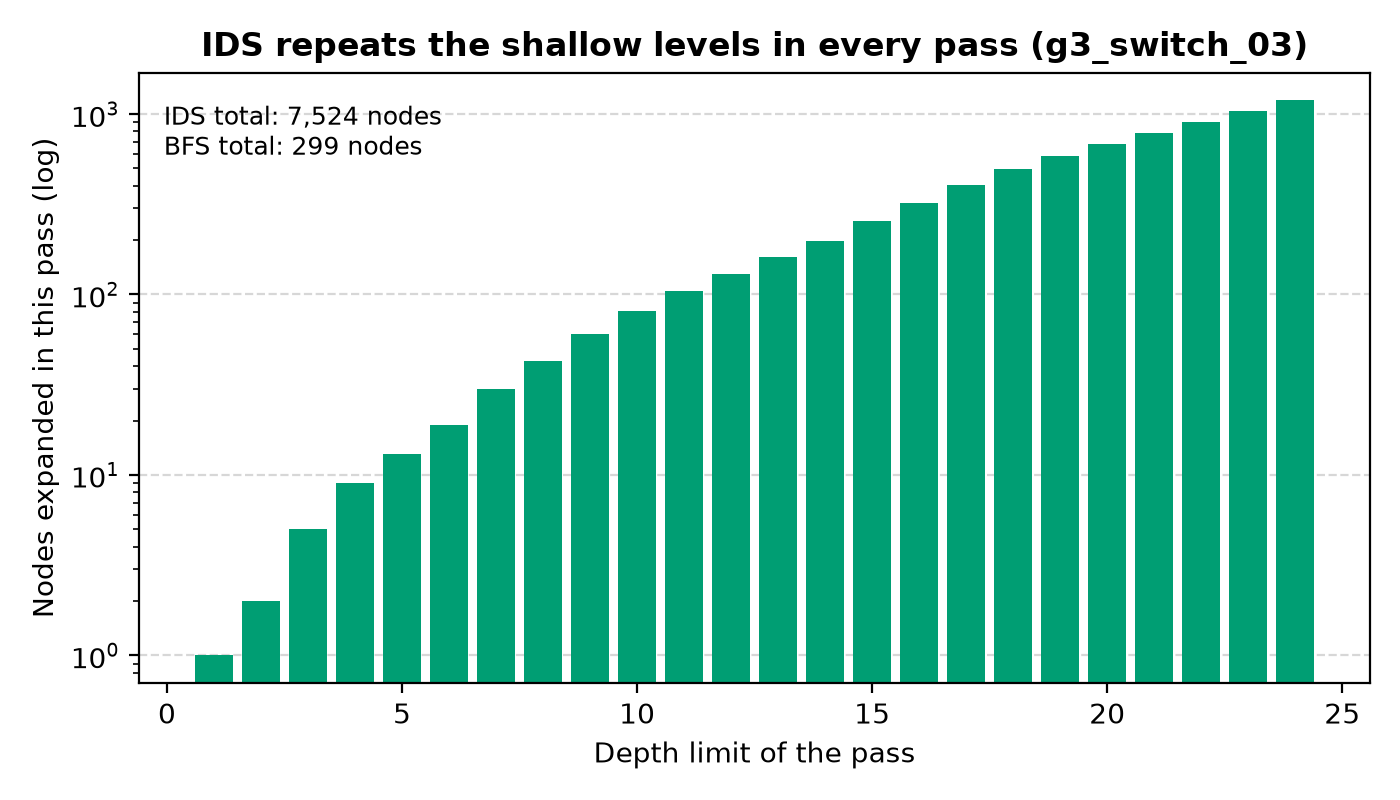
\includegraphics[width=\linewidth,height=0.45\textheight,keepaspectratio]{images/fig_ids_passes.png}
\caption{Số nút mở rộng ở từng lượt lặp của IDS trên màn g3\_switch\_03 (thang log): tổng 7.524 nút so với 299 nút của BFS. Chỉ riêng lượt cuối (giới hạn 24) đã mở rộng 1.189 nút, nhiều hơn toàn bộ BFS.}
\end{figure}

\subsubsection{Tính chất và chứng minh}

\textbf{Tính đầy đủ.} Nếu đích ở độ sâu d* (số nước đi ngắn nhất), đến lượt giới hạn d* thuật toán sẽ tìm thấy nó (chứng minh bên dưới). Nếu đích không đạt tới được, mọi lượt đều không có đích; khi giới hạn đủ lớn để không còn nút nào bị cắt, thuật toán kết luận không giải được.

\textbf{Tính tối ưu theo số nước đi.} Khẳng định: sau lượt giới hạn L, mọi trạng thái có khoảng cách ngắn nhất k ≤ L đều đã được đưa vào ngăn xếp ít nhất một lần với độ sâu đúng bằng k. Chứng minh bằng quy nạp theo k: s0 có độ sâu 0. Nếu s có khoảng cách k+1 ≤ L thì tồn tại nút cha p có khoảng cách k, được đưa vào với độ sâu k theo giả thiết và được lấy ra mở rộng với độ sâu k \textless{} L (vì k \textless{} L). Khi đó s được sinh ra với độ sâu k+1. Nó được đưa vào ngăn xếp trừ khi đã có \texttt{reached[s]} ≤ k+1; mà \texttt{reached[s]} không thể nhỏ hơn khoảng cách thực k+1, nên trong cả hai trường hợp s đã được đưa vào với độ sâu k+1. Hệ quả: lượt đầu tiên tìm thấy đích là lượt L = d*, và đường đi trả về dài d* nước. Nhờ điều kiện ``độ sâu nhỏ hơn thì cho vào lại'', phép chứng minh này không bị phá bởi thứ tự duyệt kiểu DFS.

\textbf{Độ phức tạp.} Các trạng thái ở độ sâu nhỏ bị mở rộng lại ở mọi lượt, nên tổng số nút mở rộng lớn hơn BFS. Với cây có hệ số nhánh b đều, hệ số chi phí xấp xỉ b/(b−1); với đồ thị trạng thái của Bloxorz, hệ số nhánh hiệu dụng nhỏ (số nút mỗi lượt chỉ tăng khoảng 1,1 đến 1,5 lần khi giới hạn tăng thêm 1, Hình 3) nên chi phí lặp lại lớn. Thêm vào đó, một lượt với giới hạn L còn mở rộng nhiều hơn số trạng thái cách s0 tối đa L nước, do một trạng thái có thể bị mở rộng lại mỗi khi được phát hiện ở độ sâu nhỏ hơn trong cùng lượt; vì vậy lượt cuối ở Hình 3 (1.189 nút) vượt tổng của BFS (299 nút). Về bộ nhớ, \texttt{reached} và \texttt{parent} giữ mọi trạng thái của một lượt, nên IDS \textbf{không} còn bộ nhớ tuyến tính như IDS dạng cây mà cùng bậc với BFS (đo được gấp 1,2 đến 1,6 lần BFS).

\subsection{So sánh lý thuyết ba thuật toán}

{\renewcommand{\arraystretch}{1.25}
\begin{longtable}{|>{\raggedright\arraybackslash}p{0.161\linewidth}|>{\raggedright\arraybackslash}p{0.194\linewidth}|>{\raggedright\arraybackslash}p{0.200\linewidth}|>{\raggedright\arraybackslash}p{0.305\linewidth}|}
\hline
\textbf{Tiêu chí} & \textbf{BFS} & \textbf{DFS} & \textbf{IDS} \\ \hline
\endhead
\hline
\endlastfoot
Frontier & Hàng đợi FIFO & Ngăn xếp LIFO & Ngăn xếp LIFO, giới hạn độ sâu tăng dần \\ \hline
Thời điểm kiểm tra đích & Khi sinh nút con & Khi lấy ra khỏi ngăn xếp & Khi lấy ra khỏi ngăn xếp \\ \hline
Đầy đủ & Có & Có (nhờ \texttt{visited}) & Có \\ \hline
Tối ưu theo số nước đi & Có & Không & Có \\ \hline
Tối ưu theo \texttt{physics\_\allowbreak{}cost} & Không đảm bảo & Không & Không đảm bảo \\ \hline
Thời gian & O(\textbar{}S\textbar{}), chặn bởi O(b$^{d}$) & O(\textbar{}S\textbar{}) & Lớn hơn BFS nhiều lần do mở rộng lại \\ \hline
Bộ nhớ & O(\textbar{}S\textbar{}) & O(số trạng thái đã sinh) & O(\textbar{}S\textbar{}) cho mỗi lượt \\ \hline
Phát hiện màn không giải được & Có (frontier cạn) & Có (ngăn xếp cạn) & Có (lượt không bị cắt); nếu hết \texttt{max\_\allowbreak{}depth} thì chưa kết luận \\
\end{longtable}
}

\section{Tìm kiếm có chi phí: UCS, A* và heuristic}

\subsection{Tìm kiếm chi phí đều (UCS)}

\subsubsection{Ý tưởng}

UCS (Uniform-Cost Search) mở rộng các nút theo thứ tự \textbf{chi phí đường đi tích lũy tăng dần} $g(n)$. Khi chi phí mỗi bước di chuyển là không đồng nhất (ví dụ: lăn ngang tốn 1,0, dựng đứng tốn 3,0), UCS đảm bảo tìm được đường đi có \textbf{tổng chi phí nhỏ nhất}, không chỉ ít bước nhất.

\subsubsection{Cấu trúc dữ liệu}

{\renewcommand{\arraystretch}{1.25}
\begin{longtable}{|>{\raggedright\arraybackslash}p{0.306\linewidth}|>{\raggedright\arraybackslash}p{0.624\linewidth}|}
\hline
\textbf{Thành phần} & \textbf{Mô tả} \\ \hline
\endhead
\hline
\endlastfoot
\textbf{Hàng đợi ưu tiên (frontier)} & \texttt{heapq} lưu bộ $(g, \text{tie\_breaker}, s)$. \texttt{tie\_\allowbreak{}breaker} đơn điệu tăng để phá hòa khi hai nút có cùng $g$, tránh so sánh trực tiếp giữa hai đối tượng \texttt{State}. \\ \hline
\textbf{\texttt{best\_\allowbreak{}cost[s]}} & Từ điển ánh xạ mỗi trạng thái $s$ đến chi phí đường đi tốt nhất từ trạng thái đầu đến $s$ đã biết. \\ \hline
\textbf{\texttt{parent[s]}} & Lưu cặp $(\text{state}_{\text{prev}}, \text{action})$ để truy vết đường đi khi tìm thấy đích. \\
\end{longtable}
}

\subsubsection{Mã giả}

\begin{Verbatim}[breaklines=true, fontsize=\footnotesize, frame=single]
UCS(problem, cost_fn):
    frontier <- hàng đợi ưu tiên chứa (0, 0, s0)          # (g, thứ tự đưa vào, trạng thái)
    best_cost <- { s0: 0 };  parent <- { s0: None }
    trong khi frontier không rỗng:
        (g, _, s) <- lấy ra phần tử có g nhỏ nhất
        nếu g > best_cost[s]: bỏ qua                       # bản sao cũ (lazy deletion)
        nếu is_goal(s): trả về reconstruct(parent, s)      # kiểm tra đích khi lấy ra
        expanded <- expanded + 1
        với mỗi (a, s') trong successors(s):
            g' <- g + cost_fn(s, a, s')
            nếu g' < best_cost.get(s', vô cùng):
                best_cost[s'] <- g';  parent[s'] <- (s, a)
                đưa (g', thứ tự, s') vào frontier
    trả về None                                            # không có lời giải
\end{Verbatim}

\textbf{Các điểm then chốt.}

\begin{enumerate}
\item \textbf{Kiểm tra đích khi lấy ra} (không phải khi sinh): Đảm bảo nút được lấy ra khỏi hàng đợi luôn có chi phí tối ưu, vì mọi nút có chi phí thấp hơn đã được xử lý trước đó.
\item \textbf{Xóa trễ (lazy deletion)}: Thay vì cập nhật vị trí nút trong hàng đợi (tốn $O(n)$), ta cho phép nhiều bản sao của cùng một nút tồn tại trong hàng đợi. Khi lấy ra một nút có $g > \text{best\_cost}[s]$, ta bỏ qua vì đã xử lý bản sao tốt hơn trước đó. Cách tiếp cận này đơn giản hơn \texttt{decrease-key} và phù hợp với \texttt{heapq} của Python (vốn không hỗ trợ sẵn \texttt{decrease-key}).
\item \textbf{Tính đúng đắn}: UCS luôn tìm được đường đi tối ưu khi mọi chi phí bước di chuyển dương ($c(s, a, s') \ge 1{,}0$).
\end{enumerate}

\subsubsection{Hàm chi phí \texttt{physics\_\allowbreak{}cost}}

Nhóm thiết kế hàm chi phí không đồng nhất dựa trên mô hình biến thiên thế năng trọng trường của vật rắn đồng chất kích thước $1 \times 1 \times 2$:

Khi khối nằm trên mặt phẳng, độ cao ban đầu của khối tâm (trọng tâm) là $h_0 = 0{,}5$.

\begin{enumerate}
\item \textbf{Lăn ngang (nằm → nằm).} Khối lăn quanh trục là cạnh dài $2$, thiết diện vuông $1 \times 1$. Bán kính từ trục quay đến khối tâm là $R_{\text{roll}} = \sqrt{0{,}5^2 + 0{,}5^2} = \frac{\sqrt{2}}{2} \approx 0{,}7071$. Độ nâng khối tâm lớn nhất đạt đỉnh quỹ đạo tròn:
\[\Delta h_{\text{roll}} = \frac{\sqrt{2}}{2} - 0{,}5 = \frac{\sqrt{2} - 1}{2} \approx 0{,}2071 \approx 0{,}21\]
Giá trị này được chuẩn hóa làm chi phí cơ sở (\textbf{mức chuẩn = $1{,}0$}).
\item \textbf{Dựng đứng (nằm → đứng).} Khối lật quanh trục là cạnh ngắn $1$, thiết diện chữ nhật $1 \times 2$. Bán kính từ trục quay đến khối tâm là $R_{\text{stand}} = \sqrt{0{,}5^2 + 1{,}0^2} = \frac{\sqrt{5}}{2} \approx 1{,}1180$. Độ nâng khối tâm lớn nhất:
\[\Delta h_{\text{stand}} = \frac{\sqrt{5}}{2} - 0{,}5 = \frac{\sqrt{5} - 1}{2} \approx 0{,}6180 \approx 0{,}62\]
\item \textbf{Tỷ số công cơ học nâng thế năng.}
\[\frac{\Delta h_{\text{stand}}}{\Delta h_{\text{roll}}} = \frac{\sqrt{5} - 1}{\sqrt{2} - 1} \approx \frac{0{,}6180}{0{,}2071} \approx 2{,}984 \approx 3{,}0\]
\end{enumerate}

Bảng quy đổi chi phí hoàn chỉnh:

{\renewcommand{\arraystretch}{1.25}
\begin{longtable}{|>{\raggedright\arraybackslash}p{0.292\linewidth}|>{\raggedright\arraybackslash}p{0.085\linewidth}|>{\raggedright\arraybackslash}p{0.518\linewidth}|}
\hline
\textbf{Hành động} & \textbf{Chi phí} & \textbf{Công thức \& Giải thích vật lý} \\ \hline
\endhead
\hline
\endlastfoot
Lăn ngang (nằm → nằm) & $1{,}0$ & $\Delta h_{\text{roll}} = \frac{\sqrt{2}-1}{2} \approx 0{,}21$, chọn làm mức chuẩn. \\ \hline
Dựng đứng (nằm → đứng) & $3{,}0$ & $\Delta h_{\text{stand}} = \frac{\sqrt{5}-1}{2} \approx 0{,}62$, gấp $\approx 3$ lần mức chuẩn ($2{,}98 \approx 3{,}0$). \\ \hline
Lật xuống (đứng → nằm) & $1{,}0$ & Khối tâm ở độ cao $1{,}0$, quay quanh cạnh đáy lên bán kính đỉnh $R = \frac{\sqrt{5}}{2} \approx 1{,}118 \implies \Delta h \approx 0{,}118$ (khoảng $0{,}57$ lần mức chuẩn) trước khi đổ xuống. Nhóm làm tròn lên $1{,}0$ để duy trì $c_{\min} = 1{,}0$, trực tiếp bảo toàn tính chấp nhận được (admissible) cho các cận dưới $\lceil d/2 \rceil \times c_{\min}$ của heuristic A*. \\ \hline
Di chuyển khối lập phương $1\times 1$ & $1{,}0$ & Khối $1\times 1$ lăn quanh cạnh có $\Delta h = \frac{\sqrt{2}-1}{2} \approx 0{,}207$, bằng đúng mức chuẩn của bước lăn ngang khối nguyên. \\
\end{longtable}
}

Hàm chi phí này tạo ra sự khác biệt bản chất giữa UCS và BFS: UCS sẽ \textbf{ưu tiên các đường lăn ngang} thay vì dựng đứng khi cả hai đều đi được đến đích, giúp giảm tổng hao tổn năng lượng.

\subsubsection{Độ phức tạp}

\begin{itemize}
\item \textbf{Thời gian.} $O(|E| \log |V|) = O(|V| \log |V|)$
\begin{itemize}
\item Do sử dụng \textbf{xóa trễ} (không dùng thao tác \texttt{decrease-key} vốn tốn kém), mỗi cạnh chuyển trạng thái $(s, a, s')$ có thể đẩy thêm một bản sao trạng thái vào hàng đợi ưu tiên khi tìm thấy đường rẻ hơn. Kích thước tối đa của hàng đợi là $O(|E|)$, chi phí mỗi thao tác trên hàng đợi là $O(\log |E|) = O(\log |V|^2) = O(\log |V|)$.
\item Trong không gian trạng thái của Bloxorz, bậc ra của mỗi trạng thái luôn bị chặn trên bởi một hằng số nhỏ ($\deg(s) \le 4$ khi nguyên khối, và $\deg(s) \le 5$ khi tách thành 2 khối gồm tối đa 4 hướng lăn + 1 hành động \texttt{SWITCH}). Vì vậy, tổng số cạnh thỏa mãn $|E| \le 5|V| = O(|V|)$.
\item Do đó: $O(|E| \log |E|) = O(|V| \log |V|)$.
\end{itemize}
\item \textbf{Không gian.} $O(|E|) = O(|V|)$ cho \texttt{frontier} trong trường hợp xấu nhất, và $O(|V|)$ để lưu trữ bảng \texttt{best\_\allowbreak{}cost} cùng \texttt{parent}.
\end{itemize}

\subsection{Tìm kiếm A*}

\subsubsection{Ý tưởng}

A* là cải tiến của UCS bằng cách sử dụng hàm đánh giá:

\[f(n) = g(n) + h(n)\]

trong đó:

\begin{itemize}
\item $g(n)$: chi phí đường đi thực tế từ trạng thái đầu đến $n$.
\item $h(n)$: \textbf{ước lượng} chi phí còn lại từ $n$ đến đích.
\end{itemize}

Nếu $h(n)$ thỏa tính chấp nhận được (admissible) — tức $h(n) \le h^*(n)$ với mọi $n$ — thì A* vẫn đảm bảo tìm đường đi tối ưu, nhưng mở ít nút hơn UCS nhờ ưu tiên khám phá các nút ``hứa hẹn'' gần đích hơn.

\subsubsection{Khác biệt so với UCS}

{\renewcommand{\arraystretch}{1.25}
\begin{longtable}{|l|l|l|}
\hline
\textbf{Tiêu chí} & \textbf{UCS} & \textbf{A*} \\ \hline
\endhead
\hline
\endlastfoot
Hàm ưu tiên & $g(n)$ & $f(n) = g(n) + h(n)$ \\ \hline
Heuristic & Không cần & Cần hàm $h(n)$ admissible \\ \hline
Số nút mở rộng & Nhiều hơn & Ít hơn (nhờ heuristic dẫn hướng) \\ \hline
Tính tối ưu & Luôn đảm bảo & Đảm bảo khi $h$ admissible \\
\end{longtable}
}

Cài đặt A* kế thừa cấu trúc của UCS: hàng đợi ưu tiên sắp theo $f = g + h$ thay vì $g$, và mỗi phần tử lưu thêm $g$ để phá hòa khi hai trạng thái có cùng $f$.

\subsubsection{Mã giả}

\begin{Verbatim}[breaklines=true, fontsize=\footnotesize, frame=single]
A*(problem, cost_fn, h):
    frontier <- hàng đợi ưu tiên chứa (h(s0), 0, 0, s0)   # (f, g, thứ tự đưa vào, trạng thái)
    best_g <- { s0: 0 };  parent <- { s0: None }
    trong khi frontier không rỗng:
        (f, g, _, s) <- lấy ra phần tử có f nhỏ nhất
        nếu g > best_g[s]: bỏ qua                          # bản sao cũ (lazy deletion)
        nếu is_goal(s): trả về reconstruct(parent, s)      # kiểm tra đích khi lấy ra
        expanded <- expanded + 1
        với mỗi (a, s') trong successors(s):
            g' <- g + cost_fn(s, a, s')
            nếu g' < best_g.get(s', vô cùng):
                best_g[s'] <- g';  parent[s'] <- (s, a)
                đưa (g' + h(s'), g', thứ tự, s') vào frontier
    trả về None
\end{Verbatim}

\begin{mdframed}[linecolor=blue!50!black, backgroundcolor=blue!3]
\textbf{Cơ chế phá hòa (tie-breaking) trong frontier.} Trong Python \texttt{heapq}, khi hai trạng thái có cùng giá trị hàm đánh giá $f = g + h$, bộ so sánh tuple sẽ xét đến trường thứ hai là \texttt{g\_\allowbreak{}cost}:

\begin{enumerate}
\item \textbf{Về mặt lý thuyết A* kinh điển (Russell \& Norvig - AIMA).} Khi cùng $f$, việc ưu tiên các nút có \textbf{$g$ lớn hơn} (tương đương $h$ nhỏ hơn — tức nút ở gần đích hơn) sẽ giúp thuật toán mở ít nút hơn và đi thẳng về đích nhanh hơn. Để cài đặt theo hướng này, người ta thường lưu số đối \texttt{-g\_\allowbreak{}cost} vào hàng đợi.
\item \textbf{Trong mã nguồn thực tế.} Nhóm lưu \texttt{+g\_\allowbreak{}cost} vào tuple, tức ưu tiên mở nút có $g$ nhỏ hơn trước (khám phá các đường đi an toàn có chi phí thực tích lũy thấp). Cả hai cách phá hòa đều \textbf{đảm bảo 100\% tính tối ưu nghiệm} vì $h$ thỏa mãn điều kiện admissible và consistent. Trình tự phá hòa \texttt{tie++} ở trường thứ ba đảm bảo tính ổn định (FIFO) và tránh việc Python phải so sánh trực tiếp hai đối tượng \texttt{State}.
\end{enumerate}
\end{mdframed}

\subsection{Thiết kế và phân tích tính đúng đắn của heuristic}

\subsubsection{Công thức heuristic}

Hàm heuristic $h(s)$ ước lượng chi phí còn lại từ trạng thái $s$ đến đích $G$:

\[h(s) = \begin{cases} 0 & \text{nếu } s \text{ là trạng thái đích} \\ \text{split\_cost}(c_1, c_2) & \text{nếu } s \text{ đang tách khối} \\ \max\!\big(H(s),\; c_{\text{stand}}\big) & \text{trường hợp còn lại} \end{cases}\]

với
\[H(s) = \min\!\Big(h_{\text{direct}}(s, G),\; \min_{T} \big[h_{\text{direct}}(s, T) + \text{split\_cost}(\text{targets}_T)\big]\Big)\]

Trong đó:

{\small\renewcommand{\arraystretch}{1.25}
\begin{longtable}{|>{\raggedright\arraybackslash}p{0.200\linewidth}|>{\raggedright\arraybackslash}p{0.470\linewidth}|>{\raggedright\arraybackslash}p{0.225\linewidth}|}
\hline
\textbf{Thành phần} & \textbf{Công thức} & \textbf{Ý nghĩa} \\ \hline
\endhead
\hline
\endlastfoot
$h_{\text{direct}}(s, X)$ & $\left\lceil \frac{\min_{c \in \text{cells}(s)} \text{manhattan}(c,\, X)}{2} \right\rceil \times c_{\min}$ & Cận dưới chi phí lăn khối nguyên đến ô $X$: mỗi bước lăn đi tối đa 2 ô. \\ \hline
$\text{split\_cost}(c_1, c_2)$ & $\max\!\big(\text{manhattan}(c_1, c_2) - 1,\; 0\big) \times c_{\min} + c_{\text{stand}}$ & Cận dưới chi phí để 2 khối $1\times 1$ di chuyển đến cạnh nhau (hợp nhất), sau đó dựng đứng vào đích. \\ \hline
$c_{\min}$ & $1{,}0$ & Chi phí bước đi tối thiểu (chung cho cả \texttt{physics\_\allowbreak{}cost} và \texttt{unit\_\allowbreak{}cost}). \\ \hline
$c_{\text{stand}}$ & $3{,}0$ (\texttt{physics\_\allowbreak{}cost}) hoặc $1{,}0$ (\texttt{unit\_\allowbreak{}cost}) & Chi phí tối thiểu của bước cuối cùng (dựng đứng trên ô đích). \\
\end{longtable}
}

\textbf{Giải thích trực quan.}

\begin{itemize}
\item \textbf{Nhánh trực tiếp} $h_{\text{direct}}(s, G)$: Ước lượng chi phí đi thẳng đến đích, bỏ qua mọi chướng ngại vật và cầu.
\item \textbf{Nhánh qua công tắc tách} $h_{\text{direct}}(s, T) + \text{split\_cost}(\text{targets}_T)$: Ước lượng chi phí đi đến công tắc tách $T$, rồi hai khối lập phương tìm nhau và hợp nhất.
\item Lấy $\min$ giữa các nhánh: chọn con đường ước lượng rẻ nhất.
\item Ép $\ge c_{\text{stand}}$: mọi trạng thái chưa phải đích đều cần ít nhất 1 bước dựng đứng.
\end{itemize}

\subsubsection{Chứng minh tính chấp nhận được (admissibility)}

\textbf{Định nghĩa.} $h(s)$ là admissible nếu $0 \le h(s) \le h^*(s)$ với mọi $s$, trong đó $h^*(s)$ là chi phí tối ưu thật sự.

\textbf{Chứng minh.}

\begin{enumerate}
\item \textbf{Tại đích $G$.} $h(G) = 0 = h^*(G)$.
\item \textbf{Cận dưới $c_{\text{stand}}$.} Mọi trạng thái chưa phải đích đều cần ít nhất 1 bước chuyển về đích. Bước cuối cùng buộc phải dựng khối đứng thẳng trên ô $G$, tốn tối thiểu $c_{\text{stand}}$ (3,0 với \texttt{physics\_\allowbreak{}cost}, 1,0 với \texttt{unit\_\allowbreak{}cost}). Nên $h^*(s) \ge c_{\text{stand}}$, và vì $h(s) \ge c_{\text{stand}}$ bởi phép $\max$, điều này không vi phạm.
\item \textbf{Cận dưới khoảng cách.} Khối $1\times 1\times 2$ lăn tối đa 2 ô mỗi bước, nên $\lceil d/2 \rceil \times c_{\min}$ luôn $\le$ chi phí thực tế. Khối $1\times 1$ di chuyển 1 ô/bước nên $\max(\text{manhattan} - 1, 0) \times c_{\min}$ cũng là cận dưới.
\item \textbf{Phép $\min$ bảo toàn admissibility.} $h_{\text{direct}}(s, G) \le h^*(s)$ (đường thẳng luôn $\le$ đường thực tế qua chướng ngại vật). Tương tự, chi phí qua $T$ cũng là cận dưới vì bỏ qua chướng ngại vật. Lấy $\min$ của nhiều cận dưới vẫn là cận dưới.
\end{enumerate}

\textbf{Kiểm chứng thực nghiệm.} Sử dụng Dijkstra ngược (multi-source backward Dijkstra từ mọi trạng thái đích) để tính $h^*(s)$ chính xác cho mọi trạng thái $s$ có thể chạm tới. Kiểm tra trên toàn bộ 16 màn: \textbf{0 trạng thái vi phạm} $h(s) > h^*(s)$ trên cả \texttt{physics\_\allowbreak{}cost} và \texttt{unit\_\allowbreak{}cost}.

\subsubsection{Chứng minh tính nhất quán (consistency)}

\textbf{Định nghĩa.} $h(s)$ là consistent (monotone) nếu với mọi bước chuyển $s \xrightarrow{a} s'$:

\[h(s) \le c(s, a, s') + h(s'), \quad \text{và}\quad h(G) = 0\]

Tương đương: $h(s) - h(s') \le c(s, a, s')$ — heuristic không giảm quá nhanh so với chi phí thực.

\textbf{Chứng minh qua toàn bộ 5 lớp bước chuyển trong Bloxorz.}

\textbf{1. Lăn khối nguyên (khối nguyên → khối nguyên).}

\begin{itemize}
\item Lăn khối $1\times 1\times 2$ thay đổi khoảng cách Manhattan tối thiểu đến bất kỳ ô mục tiêu $X$ nào tối đa 2 ô ($\Delta d \le 2$).
\item Do đó, $\lceil \text{dist}(s, X) / 2 \rceil$ giảm tối đa 1 mỗi bước lăn.
\item Mỗi nhánh ứng viên trong $h(s)$ giảm tối đa $c_{\min} \le c(s, a, s')$. Vì toán tử $\min/\max$ bảo toàn cận trên của hiệu, ta có $h(s) - h(s') \le c_{\min}$.
\item Trường hợp đặc biệt vào đích ($s' = G$): Bước cuối bắt buộc dựng đứng nên $c(s, a, G) \ge c_{\text{stand}}$. Tại 1 bước cách đích, $h(s) = c_{\text{stand}}$ và $h(G) = 0$, cho $h(s) - h(G) = c_{\text{stand}} \le c(s, a, G)$.
\end{itemize}

\textbf{2. Kích hoạt công tắc tách (khối nguyên $s$ → khối tách $s'$, khi dựng đứng trên $T$).}

\begin{itemize}
\item Bước lăn đứng lên $T$ chỉ xảy ra khi khối ở đủ gần nên $h_{\text{direct}}(s, T) \le c(s, a, s')$.
\item Khi đứng trên $T$, khối bị tách đến vị trí cố định $(t_1, t_2)$, nên $h(s') = \text{split\_cost}((t_1, t_2))$.
\item Vì $h_{\text{direct}}(s, T) + \text{split\_cost}((t_1, t_2))$ là một trong các nhánh ứng viên trong phép $\min(.)$ định nghĩa $h(s)$:
\end{itemize}

\[h(s) \le h_{\text{direct}}(s, T) + h(s') \implies h(s) - h(s') \le h_{\text{direct}}(s, T) \le c(s, a, s').\]

\textbf{3. Di chuyển một khối lập phương (khối tách $s$ → khối tách $s'$).}

\begin{itemize}
\item Một khối $1\times 1$ di chuyển 1 ô với chi phí $c(s, a, s') = c_{\min}$, thay đổi khoảng cách Manhattan giữa 2 khối tối đa 1 ô.
\item Dưới heuristic nới lỏng $h(s) = \max(|c_1 - c_2| - 1, 0) \times c_{\min} + c_{\text{stand}}$ (cố ý nới lỏng khoảng cách đến đích để bảo toàn tính đơn điệu), $h(s)$ giảm tối đa $1 \times c_{\min} = c_{\min} = c(s, a, s')$.
\end{itemize}

\textbf{4. Hợp nhất khối (khối tách $s$ → khối nguyên $s'$).}

\begin{itemize}
\item Theo luật trò chơi (mục 3.4.3), hai khối lập phương tự động hợp nhất thành khối nằm $1\times 1\times 2$ ngay khi vừa trở thành kề nhau; việc lăn đè lên khối kia là nước đi không hợp lệ (mục 3.4.2).
\item Do đó, ngay trước bước ghép, khoảng cách Manhattan giữa hai khối luôn là $|c_1 - c_2| = 2$.
\item Khi đó: $h(s) = \max(2 - 1, 0) \times c_{\min} + c_{\text{stand}} = c_{\min} + c_{\text{stand}}$.
\item Khối sau khi hợp nhất là trạng thái nằm $s'$ (chưa thể là đích $G$ vì vào đích buộc phải đứng), do đó $h(s') \ge c_{\text{stand}}$.
\item Suy ra:
\end{itemize}

\[h(s) - h(s') \le (c_{\min} + c_{\text{stand}}) - c_{\text{stand}} = c_{\min} \le c(s, a, s').\]

\textbf{5. Chuyển khối điều khiển (khối tách $s$ → khối tách $s'$ qua \texttt{Action.SWITCH}).}

\begin{itemize}
\item Hành động đổi khối điều khiển chiếm 28.652 / 123.355 cạnh của đồ thị. Hành động này chỉ thay đổi chỉ số khối được chọn điều khiển, vị trí tọa độ của cả 2 khối hoàn toàn giữ nguyên.
\item Do hàm \texttt{split\_\allowbreak{}cost} chỉ phụ thuộc vào khoảng cách Manhattan giữa hai khối $|c_1 - c_2|$, giá trị heuristic không đổi: $h(s') = h(s)$.
\item Suy ra:
\end{itemize}

\[h(s) - h(s') = 0 \le c(s, a, s').\]

\textbf{Kết luận.} Cả 5 lớp bước chuyển đều thỏa $h(s) - h(s') \le c(s, a, s')$, cùng với $h(G) = 0$, nên heuristic nhất quán.

\textbf{Kiểm chứng thực nghiệm toàn diện.} Quét kiểm tra toàn bộ 123.355 cạnh chuyển trạng thái có thể đạt tới (bao gồm 28.652 bước \texttt{Action.SWITCH}) trên cả 16 màn chính thức: \textbf{0 cạnh vi phạm} bất đẳng thức tam giác $h(s) \le c(s, a, s') + h(s')$ trên cả \texttt{physics\_\allowbreak{}cost} và \texttt{unit\_\allowbreak{}cost}.

\begin{mdframed}[linecolor=blue!50!black, backgroundcolor=blue!3]
\textbf{Ý nghĩa của tính nhất quán (consistent).} Với heuristic consistent, A* đảm bảo rằng mỗi nút khi được lấy ra khỏi hàng đợi ưu tiên thì $g(n)$ đã là tối ưu, nên \textbf{không bao giờ cần cập nhật lại} (re-open) bất kỳ nút nào. Điều này mạnh hơn chỉ admissible, giúp A* chạy hiệu quả hơn.
\end{mdframed}

\section{Thực nghiệm}

\subsection{Bộ kiểm thử và môi trường}

\textbf{Bộ kiểm thử cố định} gồm 16 màn trong thư mục \texttt{Source/levels/}, chia thành 4 nhóm theo độ khó tăng dần, mỗi nhóm 4 màn (Hình 1). Mọi giải thuật chạy trên đúng cùng bộ màn này và mọi màn đều giải được (đã kiểm chứng bằng BFS).

{\renewcommand{\arraystretch}{1.25}
\begin{longtable}{|>{\raggedright\arraybackslash}p{0.098\linewidth}|>{\raggedright\arraybackslash}p{0.600\linewidth}|>{\raggedright\arraybackslash}p{0.196\linewidth}|}
\hline
\textbf{Nhóm} & \textbf{Đặc điểm} & \textbf{Màn} \\ \hline
\endhead
\hline
\endlastfoot
g1 & Cơ bản: chỉ có ô sàn thường, ô trống và ô đích & \texttt{g1\_\allowbreak{}basic\_\allowbreak{}01..04} \\ \hline
g2 & Có ô dễ vỡ (khối đứng lên sẽ rơi) & \texttt{g2\_\allowbreak{}fragile\_\allowbreak{}01..04} \\ \hline
g3 & Có công tắc và cầu (mềm, nặng, tách khối; đảo hoặc cố định trạng thái cầu) & \texttt{g3\_\allowbreak{}switch\_\allowbreak{}01..04} \\ \hline
g4 & Kết hợp ô dễ vỡ, công tắc, cầu và tách khối & \texttt{g4\_\allowbreak{}combined\_\allowbreak{}01..04} \\
\end{longtable}
}

\textbf{Môi trường chạy:} Intel Core i3-1115G4 @ 3,0 GHz (4 luồng), khoảng 8 GB RAM, Linux, Python 3.14.7.

Tổng cộng 16 màn × 5 giải thuật (BFS, DFS, IDS, UCS, A*) = 80 lượt chạy; \textbf{tất cả đều giải được}, không có lượt nào vượt giới hạn thời gian.

\subsection{Phương pháp đo hiệu năng}

Bốn chỉ số được ghi nhận cho mỗi lượt chạy, theo yêu cầu của đề bài:

{\renewcommand{\arraystretch}{1.25}
\begin{longtable}{|>{\raggedright\arraybackslash}p{0.229\linewidth}|>{\raggedright\arraybackslash}p{0.701\linewidth}|}
\hline
\textbf{Chỉ số} & \textbf{Cách đo} \\ \hline
\endhead
\hline
\endlastfoot
Thời gian tìm kiếm & \texttt{time.perf\_\allowbreak{}counter()} (đồng hồ độ phân giải cao, đơn điệu, không bị ảnh hưởng khi đổi giờ hệ thống) \\ \hline
Bộ nhớ đỉnh & \texttt{tracemalloc}, trừ đi mức bộ nhớ đã cấp phát lúc bắt đầu tìm kiếm để không tính phần chuẩn bị trước đó \\ \hline
Số nút mở rộng & Theo định nghĩa ở mục 4.1, đếm qua \texttt{MetricsTracker.count\_\allowbreak{}expansion()} \\ \hline
Độ dài lời giải & Số hành động của đường đi trả về \\
\end{longtable}
}

Ngoài ra, mỗi lời giải còn được gán một giá trị \textbf{cost} bằng tổng \texttt{physics\_\allowbreak{}cost} của đường đi, tính chung một thang cho mọi giải thuật để so sánh được cả với UCS và A*.

Ba biện pháp đảm bảo độ tin cậy của phép đo (Sơ đồ 7):

\begin{enumerate}
\item \textbf{Mỗi lần đo chạy trong một tiến trình con riêng} với giới hạn thời gian (mặc định 30 giây). Cách này dùng được trên mọi hệ điều hành (không phụ thuộc \texttt{SIGALRM}) và tiến trình bị dừng hẳn khi quá hạn.
\item \textbf{Thời gian và bộ nhớ được đo ở hai lần chạy riêng.} \texttt{tracemalloc} làm chậm chương trình khoảng 3 đến 4 lần nên thời gian được đo khi tắt nó; bộ nhớ đỉnh được đo ở một lần chạy bật nó.
\item \textbf{Các lượt chạy nhanh (dưới 1 giây) được lặp lại} (mặc định 3 lần) và lấy \textbf{trung vị}, vì màn nhỏ chạy chỉ vài mili giây nên một mẫu đơn lẻ chủ yếu là nhiễu.
\end{enumerate}

\begin{sodo}[!htbp]
\centering
\caption{Quy trình đo một cặp (màn, giải thuật)}
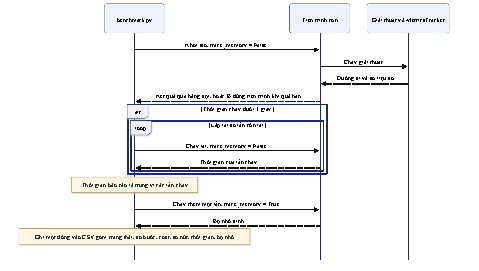
\includegraphics[width=0.95\linewidth,height=0.62\textheight,keepaspectratio]{images/sodo7.pdf}
\end{sodo}

\subsection{Quan sát trực quan cách các giải thuật duyệt không gian}

Hình 4 đặt BFS, DFS và IDS cạnh nhau trên cùng một màn nhỏ (g1\_basic\_03). Màu của mỗi ô cho biết thời điểm ô đó lần đầu bị một trạng thái được mở rộng chiếm giữ (vàng là sớm, tím là muộn); đường đen là lời giải được trả về.

\begin{figure}[!htbp]
\centering
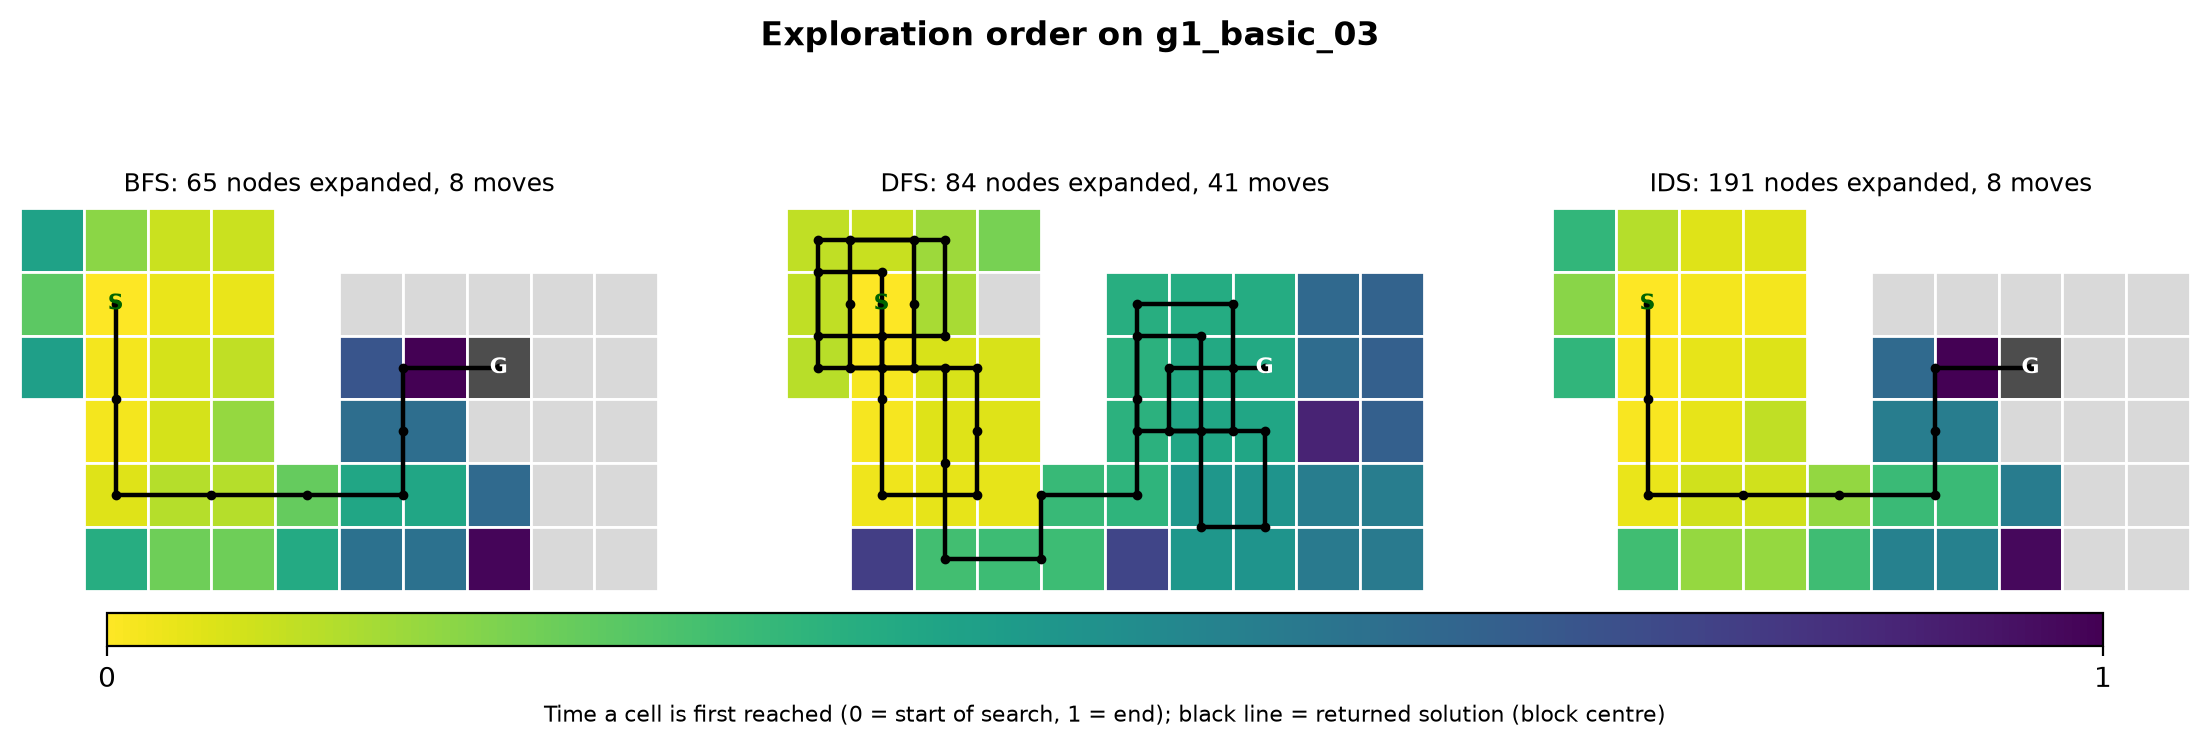
\includegraphics[width=\linewidth,height=0.45\textheight,keepaspectratio]{images/fig_exploration_order.png}
\caption{Thứ tự khám phá bàn chơi và lời giải của BFS (65 nút, 8 nước), DFS (84 nút, 41 nước) và IDS (191 nút, 8 nước) trên màn g1\_basic\_03.}
\end{figure}

Các quan sát từ hình:

\begin{itemize}
\item \textbf{BFS} lan đều theo mọi hướng từ ô xuất phát như một vết loang, nên màu chuyển dần từ vàng sang tím theo khoảng cách đến ô xuất phát, và đường đi ngắn gọn.
\item \textbf{DFS} đi sâu vào một vùng rồi quay lui. Phần bên trái của bàn bị đi đi lại lại nhiều lần trước khi sang được phía bên phải, dẫn tới lời giải 41 nước, dài hơn 5 lần lời giải tối ưu. Số nút mở rộng (84) còn lớn hơn BFS (65) trên màn này.
\item \textbf{IDS} cho cùng lời giải với BFS nhưng phải mở rộng 191 nút, gấp khoảng 3 lần BFS, do các lượt lặp.
\end{itemize}

\subsection{Bảng số liệu tổng hợp theo nhóm}

Các giá trị là \textbf{trung bình nhân} trên 4 màn của mỗi nhóm. Trung bình nhân được chọn vì số nút mở rộng trải qua nhiều bậc độ lớn giữa các màn; trung bình cộng sẽ bị một màn khó nhất (\texttt{g4\_\allowbreak{}combined\_\allowbreak{}04}) chi phối. UCS và A* được đưa vào để đối chiếu.

{\small\renewcommand{\arraystretch}{1.25}
\begin{longtable}{|l|l|r|r|r|r|r|}
\hline
\textbf{Nhóm} & \textbf{\makecell{Giải\\ thuật}} & \textbf{\makecell{Số\\ bước}} & \textbf{Cost} & \textbf{\makecell{Số nút\\ mở rộng}} & \textbf{\makecell{Thời gian\\ (ms)}} & \textbf{\makecell{Bộ nhớ\\ đỉnh (KB)}} \\ \hline
\endhead
\hline
\endlastfoot
g1 & BFS & 11,0 & 17,7 & 49 & 1,23 & 13,5 \\ \hline
g1 & DFS & 24,7 & 39,2 & 46 & 1,10 & 17,0 \\ \hline
g1 & IDS & 11,0 & 17,7 & 252 & 5,02 & 16,2 \\ \hline
g1 & UCS & 11,3 & 17,3 & 56 & 1,69 & 17,5 \\ \hline
g1 & A* & 11,3 & 17,3 & 46 & 1,58 & 16,0 \\ \hline
g2 & BFS & 21,6 & 33,8 & 78 & 1,85 & 21,4 \\ \hline
g2 & DFS & 30,9 & 48,9 & 53 & 1,31 & 19,7 \\ \hline
g2 & IDS & 21,6 & 33,8 & 1.501 & 26,15 & 29,6 \\ \hline
g2 & UCS & 22,0 & 33,4 & 83 & 1,98 & 27,5 \\ \hline
g2 & A* & 22,0 & 33,4 & 78 & 1,84 & 26,1 \\ \hline
g3 & BFS & 18,5 & 33,1 & 199 & 4,09 & 60,1 \\ \hline
g3 & DFS & 70,1 & 116,4 & 178 & 3,38 & 71,5 \\ \hline
g3 & IDS & 18,5 & 33,1 & 2.833 & 51,19 & 85,5 \\ \hline
g3 & UCS & 18,6 & 32,9 & 239 & 4,70 & 86,1 \\ \hline
g3 & A* & 18,6 & 32,9 & 198 & 4,34 & 75,1 \\ \hline
g4 & BFS & 22,8 & 33,6 & 2.836 & 46,79 & 942,3 \\ \hline
g4 & DFS & 114,5 & 162,7 & 171 & 3,61 & 98,8 \\ \hline
g4 & IDS & 22,8 & 33,6 & 48.008 & 819,42 & 1.398,7 \\ \hline
g4 & UCS & 22,8 & 33,6 & 5.290 & 99,74 & 1.866,8 \\ \hline
g4 & A* & 22,8 & 33,6 & 3.041 & 55,85 & 1.273,1 \\
\end{longtable}
}

Bảng chi tiết nhóm khó nhất (g4), nơi các giải thuật phân biệt rõ nhất:

{\small\renewcommand{\arraystretch}{1.25}
\begin{longtable}{|l|l|r|r|r|r|r|}
\hline
\textbf{Màn} & \textbf{\makecell{Giải\\ thuật}} & \textbf{\makecell{Số\\ bước}} & \textbf{Cost} & \textbf{\makecell{Số nút\\ mở rộng}} & \textbf{\makecell{Thời gian\\ (ms)}} & \textbf{\makecell{Bộ nhớ\\ đỉnh (KB)}} \\ \hline
\endhead
\hline
\endlastfoot
g4\_combined\_01 & BFS & 12 & 22 & 242 & 3,88 & 108,0 \\ \hline
g4\_combined\_01 & DFS & 24 & 42 & 42 & 0,96 & 16,6 \\ \hline
g4\_combined\_01 & IDS & 12 & 22 & 1.175 & 19,48 & 135,4 \\ \hline
g4\_combined\_02 & BFS & 29 & 39 & 4.597 & 74,68 & 1.233,2 \\ \hline
g4\_combined\_02 & DFS & 304 & 376 & 390 & 9,11 & 273,8 \\ \hline
g4\_combined\_02 & IDS & 29 & 39 & 104.403 & 1.906,44 & 1.949,9 \\ \hline
g4\_combined\_03 & BFS & 25 & 33 & 5.228 & 96,73 & 1.719,6 \\ \hline
g4\_combined\_03 & DFS & 141 & 181 & 224 & 5,21 & 147,4 \\ \hline
g4\_combined\_03 & IDS & 25 & 33 & 100.085 & 1.745,56 & 2.652,8 \\ \hline
g4\_combined\_04 & BFS & 31 & 45 & 11.118 & 171,15 & 3.444,0 \\ \hline
g4\_combined\_04 & DFS & 167 & 245 & 234 & 3,75 & 142,6 \\ \hline
g4\_combined\_04 & IDS & 31 & 45 & 432.630 & 6.954,95 & 5.465,3 \\
\end{longtable}
}

Bảng đầy đủ cho cả 16 màn và 5 giải thuật được đưa vào Phụ lục A.

\begin{figure}[!htbp]
\centering
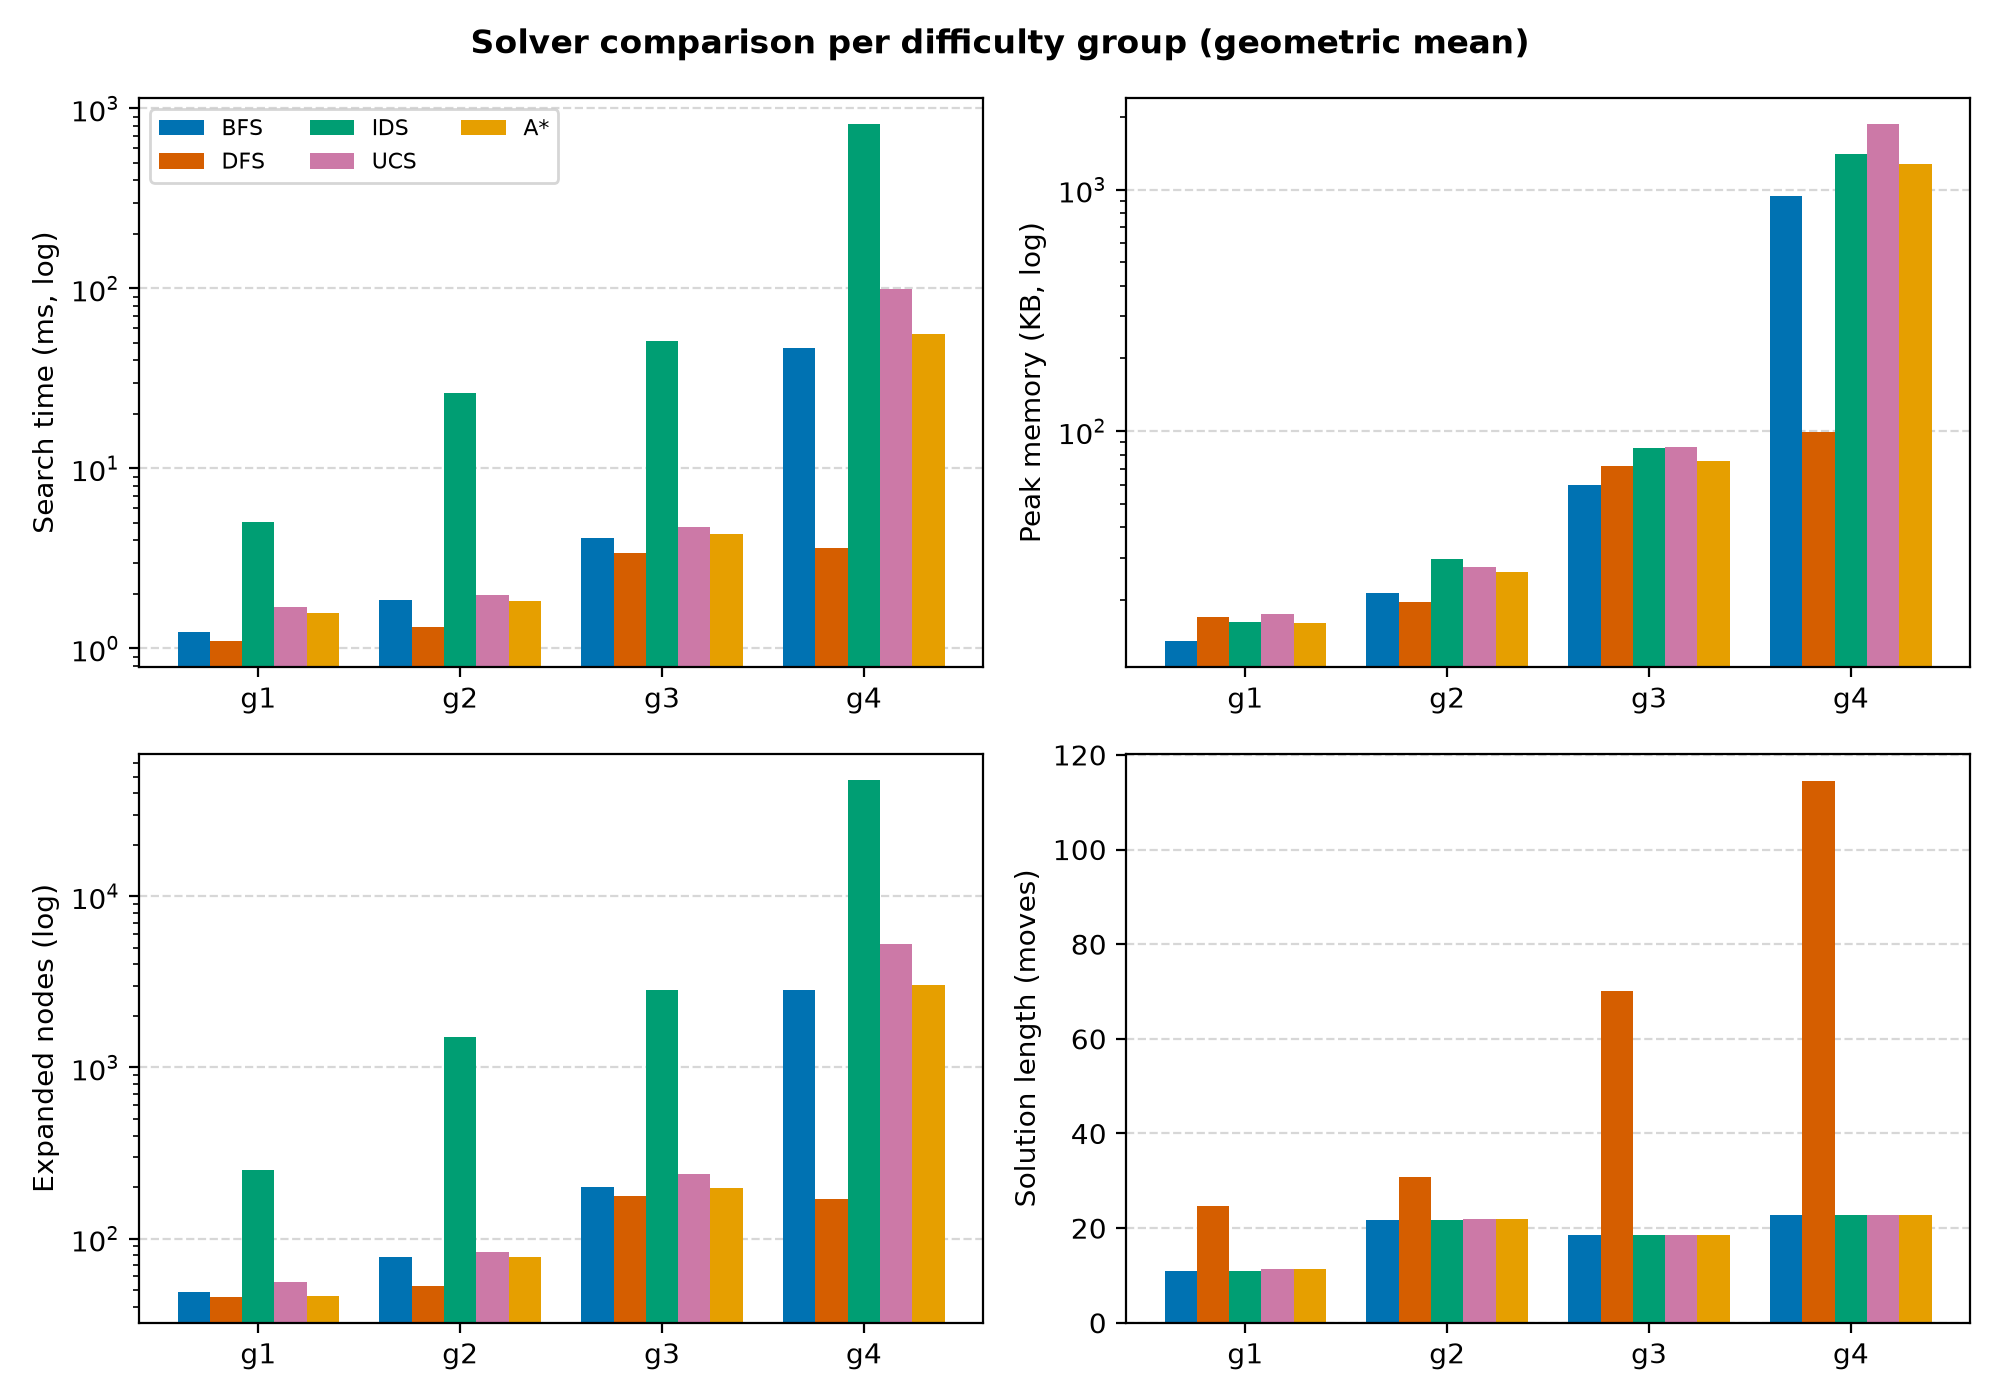
\includegraphics[width=\linewidth,height=0.45\textheight,keepaspectratio]{images/fig_metrics_by_group.png}
\caption{Thời gian, bộ nhớ, số nút mở rộng (thang log) và độ dài lời giải theo nhóm màn (trung bình nhân).}
\end{figure}

\begin{figure}[!htbp]
\centering
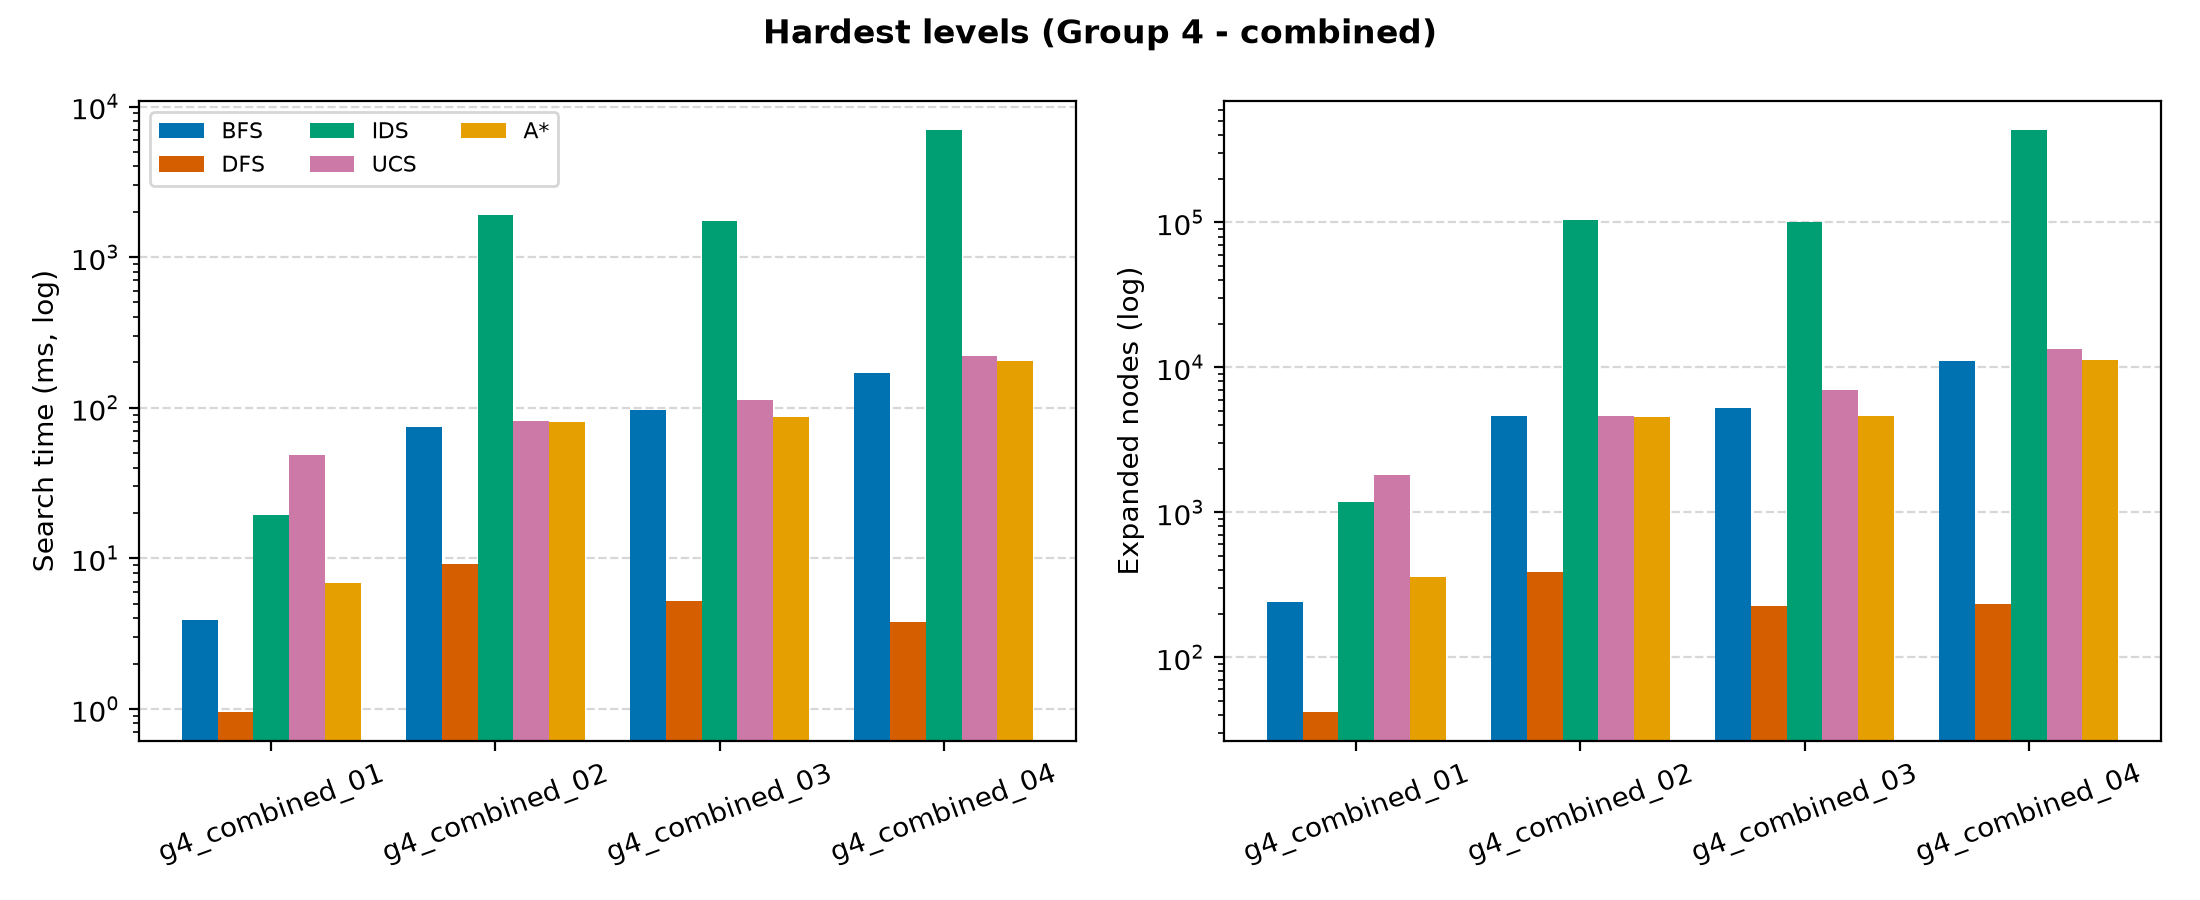
\includegraphics[width=\linewidth,height=0.45\textheight,keepaspectratio]{images/fig_hardest_levels.png}
\caption{Thời gian và số nút mở rộng trên 4 màn khó nhất (nhóm g4), thang log.}
\end{figure}

\subsection{Nhận xét}

\textbf{Chất lượng lời giải.}

\begin{itemize}
\item BFS và IDS cho \textbf{đúng cùng số bước ở cả 16 màn}, và đó là số bước nhỏ nhất, phù hợp với phần chứng minh ở mục 4.2.6 và 4.4.6.
\item Số bước nhỏ nhất \textbf{chưa chắc là cost nhỏ nhất}. Ở 3/16 màn, UCS và A* tìm được lời giải có cost thấp hơn dù nhiều bước hơn: \texttt{g1\_\allowbreak{}basic\_\allowbreak{}03} (BFS 8 bước, cost 14; UCS 9 bước, cost 13), \texttt{g2\_\allowbreak{}fragile\_\allowbreak{}01} (16 bước, cost 24; so với 17 bước, cost 23) và \texttt{g3\_\allowbreak{}switch\_\allowbreak{}04} (23 bước, cost 41; so với 24 bước, cost 40). Mức vượt trung bình chỉ 0,6 đến 1,9\% ở g1–g3 và 0\% ở g4 (Hình 7). Hai thước đo ``số nước đi'' và \texttt{physics\_\allowbreak{}cost} trùng nhau ở hầu hết các màn nhưng không phải luôn luôn, nên BFS và IDS tối ưu theo số nước đi mà không đảm bảo tối ưu theo cost.
\item DFS là giải thuật duy nhất cho lời giải \textbf{kém hẳn}: dài gấp 1,0 đến 10,5 lần lời giải ngắn nhất (trung vị khoảng 3,1 lần) và chỉ đạt cost tối ưu ở 1/16 màn (\texttt{g2\_\allowbreak{}fragile\_\allowbreak{}02}). Ở g4 lời giải trung bình là 114,5 nước so với 22,8 nước, cost cao hơn khoảng 384\%. Màn tệ nhất là \texttt{g4\_\allowbreak{}combined\_\allowbreak{}02}: 304 nước so với 29 nước tối ưu.
\end{itemize}

\begin{figure}[!htbp]
\centering
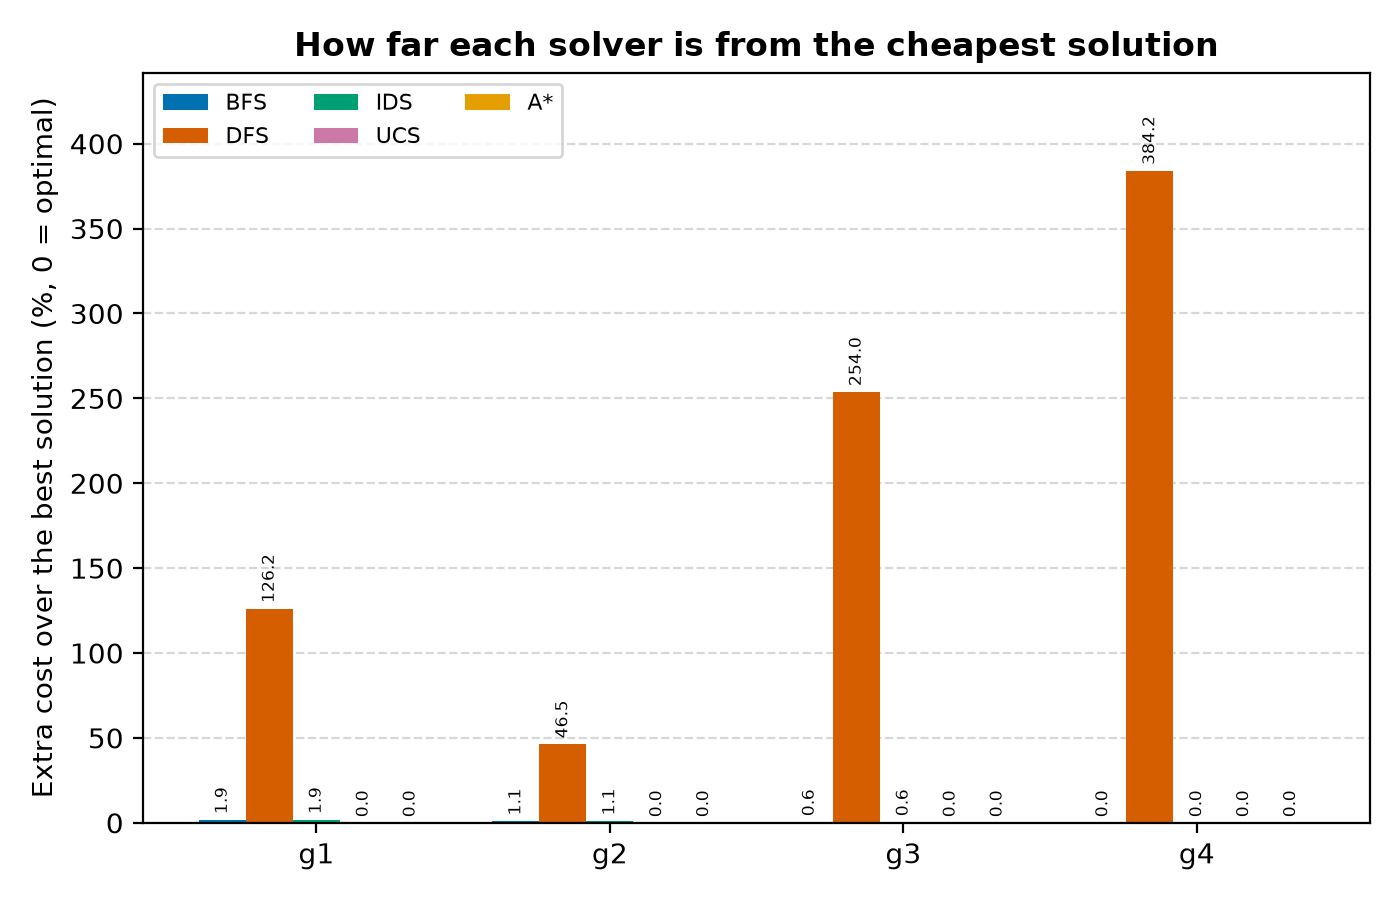
\includegraphics[width=\linewidth,height=0.45\textheight,keepaspectratio]{images/fig_cost_ratio.png}
\caption{Phần trăm cost vượt so với cost thấp nhất tìm được trên mỗi màn (0 nghĩa là tối ưu theo \texttt{physics\_\allowbreak{}cost}).}
\end{figure}

\textbf{Chi phí tìm kiếm.}

\begin{itemize}
\item \textbf{DFS} mở rộng ít nút hơn BFS ở 12/16 màn và nhanh nhất ở nhóm g4 (3,6 ms so với 46,8 ms của BFS), vì nó đi thẳng theo một nhánh mà không phải duyệt hết từng lớp. Đổi lại lời giải rất dài, và kết quả phụ thuộc vào thứ tự hành động cố định U, D, L, R: đổi thứ tự có thể cho kết quả khác hẳn. Ưu thế về tốc độ của DFS vì vậy mang tính may rủi chứ không phải được đảm bảo; Hình 4 cho thấy trên màn g1\_basic\_03 DFS thậm chí mở rộng nhiều nút hơn BFS.
\item \textbf{BFS} có số nút mở rộng tăng nhanh theo độ khó (49 nút ở g1 lên 2.836 nút ở g4, tăng khoảng 58 lần), vì số trạng thái tăng mạnh khi có thêm ô đặc biệt, cầu (mỗi cầu làm số cấu hình cầu có thể tăng tới gấp đôi) và khối tách.
\item \textbf{IDS} tốn kém nhất: mở rộng nhiều hơn BFS từ \textbf{2,9 đến 38,9 lần} và chậm hơn từ 2,6 đến 40,6 lần. Ở \texttt{g4\_\allowbreak{}combined\_\allowbreak{}04} IDS mở rộng 432.630 nút (so với 11.118 nút của BFS) và mất khoảng 7 giây. Nguyên nhân là mỗi lượt lặp mở rộng lại toàn bộ các trạng thái ở độ sâu nhỏ hơn (Hình 3); chênh lệch càng lớn khi lời giải càng sâu.
\end{itemize}

\textbf{Bộ nhớ.}

\begin{itemize}
\item Nhận định thường gặp ``DFS và IDS tốn ít bộ nhớ hơn BFS'' chỉ đúng với tìm kiếm dạng cây. Ở đây cả ba là tìm kiếm trên đồ thị nên đều phải giữ bảng các trạng thái đã thăm, và kết quả đo cho thấy:
\begin{itemize}
\item \textbf{IDS dùng nhiều bộ nhớ hơn BFS ở cả 16 màn} (gấp 1,2 đến 1,6 lần) do bảng \texttt{reached} và \texttt{parent} cộng thêm ngăn xếp.
\item \textbf{DFS dùng ít bộ nhớ hơn BFS ở 7/16 màn}, trong đó có cả 4 màn g4 (98,8 KB so với 942,3 KB). Nhưng ở nhiều màn nhỏ DFS dùng \emph{nhiều hơn} BFS (như \texttt{g1\_\allowbreak{}basic\_\allowbreak{}03}: 39,0 KB so với 20,3 KB), vì DFS đưa tất cả nút con vào ngăn xếp và \texttt{visited} trước khi quyết định đi tiếp. Ở g4 DFS tiết kiệm bộ nhớ chủ yếu vì nó tìm thấy đích chỉ sau khoảng 170 lần mở rộng, chứ không phải nhờ cấu trúc bộ nhớ tốt hơn.
\end{itemize}
\item Bộ nhớ của BFS tăng khoảng 70 lần từ g1 đến g4 (13,5 KB lên 942,3 KB), cùng xu hướng với số nút; DFS chỉ tăng khoảng 6 lần (17,0 KB lên 98,8 KB) vì số nút nó khám phá gần như không đổi.
\end{itemize}

\textbf{Theo nhóm độ khó.} Ở g1 và g2 (màn nhỏ), cả năm giải thuật đều chạy dưới 50 ms nên chênh lệch tuyệt đối không đáng kể dù IDS đã chậm hơn BFS hàng chục lần về tỉ lệ. Sự khác biệt về giá trị tuyệt đối chỉ lộ rõ ở g3 và nhất là g4, nơi công tắc, cầu và khối tách làm không gian trạng thái phình lên. Vì vậy các kết luận về hiệu năng nên chủ yếu dựa vào hai nhóm này.

\subsection{So sánh UCS và A*}

\subsubsection{So sánh số đỉnh mở rộng}

\textbf{Với \texttt{physics\_\allowbreak{}cost} ($c_{\text{stand}} = 3.0$):}

{\small\renewcommand{\arraystretch}{1.25}
\begin{longtable}{|l|r|r|r|r|r|}
\hline
\textbf{Màn} & \textbf{UCS (đỉnh mở)} & \textbf{A* (đỉnh mở)} & \textbf{Chi phí ($g^*$)} & \textbf{Bước} & \textbf{Giảm} \\ \hline
\endhead
\hline
\endlastfoot
g1\_basic\_01 & 44 & 37 & 12.0 & 8 & 15.9\% \\ \hline
g1\_basic\_02 & 61 & 56 & 20.0 & 12 & 8.2\% \\ \hline
g1\_basic\_03 & 89 & 60 & 13.0 & 9 & 32.6\% \\ \hline
g1\_basic\_04 & 40 & 37 & 29.0 & 19 & 7.5\% \\ \hline
g2\_fragile\_01 & 99 & 93 & 23.0 & 17 & 6.1\% \\ \hline
g2\_fragile\_02 & 49 & 43 & 31.0 & 19 & 12.2\% \\ \hline
g2\_fragile\_03 & 94 & 87 & 38.0 & 24 & 7.4\% \\ \hline
g2\_fragile\_04 & 106 & 104 & 46.0 & 30 & 1.9\% \\ \hline
g3\_switch\_01 & 203 & 187 & 29.0 & 15 & 7.9\% \\ \hline
g3\_switch\_02 & 130 & 95 & 24.0 & 14 & 26.9\% \\ \hline
g3\_switch\_03 & 374 & 309 & 42.0 & 24 & 17.4\% \\ \hline
g3\_switch\_04 & 333 & 281 & 40.0 & 24 & 15.6\% \\ \hline
g4\_combined\_01 & 1,816 & 357 & 22.0 & 12 & \textbf{80.3\%} \\ \hline
g4\_combined\_02 & 4,641 & 4,552 & 39.0 & 29 & 1.9\% \\ \hline
g4\_combined\_03 & 6,932 & 4,649 & 33.0 & 25 & 32.9\% \\ \hline
g4\_combined\_04 & 13,405 & 11,315 & 45.0 & 31 & 15.6\% \\ \hline
\textbf{Tổng cộng} & \textbf{28,416} & \textbf{22,262} & — & — & \textbf{21.7\%} \\
\end{longtable}
}

\emph{(Ghi chú: UCS và A* tìm ra kết quả đồng nhất cả về tổng chi phí tối ưu $g^*$ lẫn số bước đi trên mọi màn).}

\textbf{Với \texttt{unit\_\allowbreak{}cost} ($c_{\text{stand}} = 1.0$):}

{\small\renewcommand{\arraystretch}{1.25}
\begin{longtable}{|l|r|r|r|r|r|}
\hline
\textbf{Màn} & \textbf{UCS (đỉnh mở)} & \textbf{A* (đỉnh mở)} & \textbf{Chi phí ($g^*$)} & \textbf{Bước} & \textbf{Giảm} \\ \hline
\endhead
\hline
\endlastfoot
g1\_basic\_01 & 44 & 37 & 8.0 & 8 & 15.9\% \\ \hline
g1\_basic\_02 & 62 & 52 & 12.0 & 12 & 16.1\% \\ \hline
g1\_basic\_03 & 84 & 47 & 8.0 & 8 & \textbf{44.0\%} \\ \hline
g1\_basic\_04 & 40 & 40 & 19.0 & 19 & 0.0\% \\ \hline
g2\_fragile\_01 & 101 & 96 & 16.0 & 16 & 5.0\% \\ \hline
g2\_fragile\_02 & 45 & 41 & 19.0 & 19 & 8.9\% \\ \hline
g2\_fragile\_03 & 93 & 85 & 24.0 & 24 & 8.6\% \\ \hline
g2\_fragile\_04 & 105 & 104 & 30.0 & 30 & 1.0\% \\ \hline
g3\_switch\_01 & 180 & 121 & 15.0 & 15 & 32.8\% \\ \hline
g3\_switch\_02 & 125 & 72 & 14.0 & 14 & \textbf{42.4\%} \\ \hline
g3\_switch\_03 & 342 & 263 & 24.0 & 24 & 23.1\% \\ \hline
g3\_switch\_04 & 329 & 249 & 23.0 & 23 & 24.3\% \\ \hline
g4\_combined\_01 & 360 & 83 & 12.0 & 12 & \textbf{76.9\%} \\ \hline
g4\_combined\_02 & 4,627 & 3,594 & 29.0 & 29 & 22.3\% \\ \hline
g4\_combined\_03 & 5,544 & 3,822 & 25.0 & 25 & 31.1\% \\ \hline
g4\_combined\_04 & 11,563 & 8,129 & 31.0 & 31 & 29.7\% \\ \hline
\textbf{Tổng cộng} & \textbf{23,644} & \textbf{16,835} & — & — & \textbf{28.8\%} \\
\end{longtable}
}

\subsubsection{Nhận xét}

\begin{enumerate}
\item \textbf{Tính tối ưu tuyệt đối về chi phí:} Trên toàn bộ 16 màn, A* luôn tìm được lời giải có \textbf{cùng tổng chi phí tối ưu $g^*$} (và khớp hoàn toàn số bước) với UCS. Đây là hệ quả trực tiếp của tính admissible và consistent đã được chứng minh chặt chẽ cả trên lý thuyết lẫn qua kiểm chứng thực nghiệm 123,355 cạnh.
\item \textbf{Minh chứng thực nghiệm cho hiệu ứng của \texttt{physics\_\allowbreak{}cost}:} So sánh chéo giữa hai bảng thực nghiệm, tại 3 màn \texttt{g1\_\allowbreak{}basic\_\allowbreak{}03}, \texttt{g2\_\allowbreak{}fragile\_\allowbreak{}01} và \texttt{g3\_\allowbreak{}switch\_\allowbreak{}04}, số bước trong lời giải tối ưu của \texttt{physics\_\allowbreak{}cost} dài hơn \texttt{unit\_\allowbreak{}cost} đúng 1 bước:
\begin{itemize}
\item Ở \texttt{g1\_\allowbreak{}basic\_\allowbreak{}03}: \texttt{unit\_\allowbreak{}cost} đi 8 bước (tiêu tốn $14.0$ nếu quy đổi theo physics cost), trong khi \texttt{physics\_\allowbreak{}cost} đi 9 bước (chỉ tốn $13.0$).
\item Ở \texttt{g2\_\allowbreak{}fragile\_\allowbreak{}01}: \texttt{unit\_\allowbreak{}cost} đi 16 bước (tiêu tốn $24.0$ physics cost), trong khi \texttt{physics\_\allowbreak{}cost} đi 17 bước (chỉ tốn $23.0$).
\item Ở \texttt{g3\_\allowbreak{}switch\_\allowbreak{}04}: \texttt{unit\_\allowbreak{}cost} đi 23 bước (tiêu tốn $41.0$ physics cost), trong khi \texttt{physics\_\allowbreak{}cost} đi 24 bước (chỉ tốn $40.0$).
\end{itemize}
Thuật toán UCS và A* đã chủ động chọn đường lăn ngang dài hơn 1 bước nhằm triệt tiêu bớt một bước dựng đứng tốn kém (chi phí $3.0$). Minh chứng thực tế này khẳng định hàm \texttt{physics\_\allowbreak{}cost} đã thay đổi hành vi tìm kiếm theo đúng mô hình tối ưu năng lượng cơ học đã đề ra ở mục 5.1.4.
\item \textbf{Hiệu quả tìm kiếm:} A* giảm trung bình \textbf{21.7\%} số đỉnh mở rộng so với UCS trên \texttt{physics\_\allowbreak{}cost} và \textbf{28.8\%} trên \texttt{unit\_\allowbreak{}cost}. Heuristic phát huy hiệu quả mạnh nhất trên các màn có không gian trạng thái phức tạp và phân nhánh rộng:
\begin{itemize}
\item \texttt{g4\_\allowbreak{}combined\_\allowbreak{}01}: giảm tới \textbf{80.3\%} (physics) / \textbf{76.9\%} (unit) — heuristic cắt tỉa gần như toàn bộ các nhánh đi chệch hướng khỏi mục tiêu.
\item \texttt{g3\_\allowbreak{}switch\_\allowbreak{}02}: giảm \textbf{26.9\%} (physics) / \textbf{42.4\%} (unit) — heuristic dẫn hướng hiệu quả qua các cây cầu và công tắc.
\end{itemize}
\item \textbf{Trường hợp heuristic ít cải thiện:} Trên các màn có địa hình hành lang hẹp hoặc bắt buộc chỉ có một con đường hợp lệ duy nhất:
\begin{itemize}
\item \texttt{g2\_\allowbreak{}fragile\_\allowbreak{}04}: chỉ giảm 1.9\% (physics) — bản đồ dài và hẹp, hầu hết các trạng thái sinh ra đều thuộc về tuyến đường khả dĩ duy nhất.
\item \texttt{g1\_\allowbreak{}basic\_\allowbreak{}04}: giảm 0.0\% (unit) — không gian không có nhánh cụt dư thừa để cắt tỉa.
\end{itemize}
\end{enumerate}

\subsection{Ưu điểm và nhược điểm}

{\renewcommand{\arraystretch}{1.25}
\begin{longtable}{|>{\raggedright\arraybackslash}p{0.070\linewidth}|>{\raggedright\arraybackslash}p{0.263\linewidth}|>{\raggedright\arraybackslash}p{0.263\linewidth}|>{\raggedright\arraybackslash}p{0.263\linewidth}|}
\hline
 & \textbf{Ưu điểm} & \textbf{Nhược điểm} & \textbf{Phù hợp khi} \\ \hline
\endhead
\hline
\endlastfoot
\textbf{BFS} & Đảm bảo ít nước đi nhất; đơn giản; ổn định, ít phụ thuộc thứ tự hành động & Số nút và bộ nhớ tăng nhanh theo độ khó; không đảm bảo cost tối ưu khi chi phí không đồng nhất & Cần lời giải ngắn nhất và không gian trạng thái vừa phải \\ \hline
\textbf{DFS} & Nhanh và ít nút nhất ở màn khó; mã nguồn ngắn & Lời giải rất dài (tới 10 lần); kết quả phụ thuộc thứ tự hành động; không tối ưu & Chỉ cần một lời giải bất kỳ, càng nhanh càng tốt \\ \hline
\textbf{IDS} & Tối ưu số nước như BFS; kết luận được ``không giải được'' & Chậm nhất, mở rộng nhiều nút nhất vì lặp lại; trong cài đặt trên đồ thị không tiết kiệm bộ nhớ so với BFS & Khi cần tính tối ưu và hạn chế bộ nhớ chặt (dạng cây thuần túy) \\
\end{longtable}
}

Ưu điểm và nhược điểm của UCS và A*:

\textbf{UCS}

{\renewcommand{\arraystretch}{1.25}
\begin{longtable}{|>{\raggedright\arraybackslash}p{0.447\linewidth}|>{\raggedright\arraybackslash}p{0.483\linewidth}|}
\hline
\textbf{Ưu điểm} & \textbf{Nhược điểm} \\ \hline
\endhead
\hline
\endlastfoot
Đảm bảo tối ưu với mọi hàm chi phí dương. & Không có dẫn hướng, mở rộng đều theo mọi hướng (``tìm kiếm mù''). \\ \hline
Cài đặt đơn giản, không cần heuristic. & Mở nhiều đỉnh không cần thiết trên bản đồ lớn. \\ \hline
Hoạt động đúng ngay cả khi chi phí không đồng nhất. & Hiệu suất kém hơn A* khi có heuristic tốt. \\
\end{longtable}
}

\textbf{A*}

{\renewcommand{\arraystretch}{1.25}
\begin{longtable}{|>{\raggedright\arraybackslash}p{0.465\linewidth}|>{\raggedright\arraybackslash}p{0.465\linewidth}|}
\hline
\textbf{Ưu điểm} & \textbf{Nhược điểm} \\ \hline
\endhead
\hline
\endlastfoot
Giảm đáng kể số đỉnh mở rộng so với UCS (trung bình 21–29\%). & Cần thiết kế heuristic chặt chẽ: sai sẽ mất tính tối ưu. \\ \hline
Vẫn đảm bảo tính tối ưu nhờ heuristic admissible + consistent. & Heuristic dựa trên Manhattan distance nên ít hiệu quả trên bản đồ hẹp, dài, hoặc bản đồ có nhiều cầu (khoảng cách Manhattan bị biến dạng do cầu đóng/mở làm gián đoạn đường đi thực tế). \\ \hline
Heuristic consistent → không bao giờ re-open đỉnh → hiệu quả bộ nhớ. & Trên bản đồ nhỏ (\textless{} 100 đỉnh), chi phí tính heuristic có thể không bù được lợi ích cắt tỉa. \\ \hline
Trên bản đồ lớn (g4), tiết kiệm tới 80\% số đỉnh mở rộng. & Cần điều chỉnh tham số $c_{\text{stand}}$ theo hàm chi phí (đã tự động hóa). \\
\end{longtable}
}

\subsection{Hạn chế của thực nghiệm}

\begin{itemize}
\item Mỗi nhóm chỉ có 4 màn nên trung bình nhân chỉ có ý nghĩa định tính.
\item Thời gian là trung vị của 3 lần chạy trên một máy, có thể dao động theo tải hệ thống; các màn g1–g2 chạy chỉ vài mili giây nên sai số tương đối lớn. Bộ nhớ đo bằng \texttt{tracemalloc} chỉ tính phần cấp phát bởi Python, không phải toàn bộ RAM của tiến trình.
\item Kết quả của DFS gắn với thứ tự hành động cố định và không thể khái quát cho thứ tự khác.
\end{itemize}

\section{Kết luận}

\subsection{Kết quả đạt được}

\begin{itemize}
\item Trò chơi Bloxorz chơi được trên giao diện Pygame, có đủ cơ chế cơ bản và các ô đặc biệt mà đề yêu cầu: ô dễ vỡ, cầu, công tắc mềm, nặng, tách, cùng cơ chế tách và ghép khối.
\item Bài toán được hình thức hoá với trạng thái bất biến, gồm cả cấu hình cầu và khối đang điều khiển, và một bảng chuyển tư thế được kiểm thử đủ 12 trường hợp.
\item Năm thuật toán BFS, DFS, IDS, UCS, A* được nhóm tự cài đặt, dùng chung một mô hình bài toán và một cách đo, và được so sánh trên bộ 16 màn cố định thuộc 4 nhóm độ khó.
\end{itemize}

\subsection{Nhận xét chính}

\begin{itemize}
\item \textbf{BFS là lựa chọn cân bằng nhất trong ba thuật toán không có thông tin.} BFS tối ưu theo số nước đi, mở rộng ít nút hơn IDS rất nhiều, và cho lời giải ngắn hơn hẳn DFS.
\item \textbf{DFS nhanh nhưng lời giải kém.} DFS mở rộng ít nút nhất trên các màn khó, nhưng lời giải dài gấp 1,0 đến 10,5 lần lời giải ngắn nhất và phụ thuộc thứ tự duyệt hành động.
\item \textbf{IDS cho cùng lời giải với BFS nhưng tốn kém nhất.} IDS có cùng số bước với BFS trên cả 16 màn. Nhưng IDS mở rộng nhiều hơn BFS 2,9 đến 38,9 lần, và vì được cài đặt trên đồ thị nên không còn lợi thế bộ nhớ.
\item \textbf{Hàm chi phí không đồng nhất thay đổi lời giải.} Ở 3/16 màn, UCS và A* chọn đi thêm một nước để bớt một lần dựng đứng, nên tổng \texttt{physics\_\allowbreak{}cost} thấp hơn lời giải ít nước nhất. Ít nước nhất vì vậy không đồng nghĩa với rẻ nhất.
\item \textbf{Heuristic giúp A* hiệu quả hơn UCS mà vẫn tối ưu.} A* luôn cho cùng chi phí tối ưu với UCS, và mở rộng ít hơn UCS 21,7\% số nút với \texttt{physics\_\allowbreak{}cost}, 28,8\% với \texttt{unit\_\allowbreak{}cost}. Mức giảm cao nhất là khoảng 80\% trên \texttt{g4\_\allowbreak{}combined\_\allowbreak{}01}. Heuristic đã được chứng minh chấp nhận được và nhất quán, đồng thời kiểm chứng trên toàn bộ 123 355 cạnh của 16 màn.
\end{itemize}

\subsection{Hạn chế và hướng phát triển}

\begin{itemize}
\item Bộ thử chỉ có 4 màn mỗi nhóm. Có thể mở rộng bằng các màn của trò chơi gốc hoặc sinh màn tự động để kết luận chắc chắn hơn.
\item Heuristic dựa trên khoảng cách Manhattan, nên ít hiệu quả trên màn hẹp, dài, hoặc có cầu chắn đường. Có thể thay bằng khoảng cách đường đi ngắn nhất trên lưới đã nới lỏng (bỏ qua tư thế khối), tính trước một lần cho mỗi màn.
\item IDS có thể dùng tập đường đi hiện tại thay cho bảng \texttt{reached} để giữ bộ nhớ tuyến tính theo độ sâu, đổi lại phải chấp nhận mở rộng lại nhiều hơn.
\end{itemize}


% 5. Phụ lục
\appendix
\section{Kết quả thực nghiệm đầy đủ}

Các bảng dưới đây liệt kê đủ 80 lượt chạy (16 màn × 5 thuật toán), lấy từ cùng tệp CSV với các bảng ở mục 6.4. Dấu \texttt{*} đánh dấu chi phí thấp nhất tìm được trên màn đó.

\emph{Nhóm g1 (cơ bản)}

{\small\renewcommand{\arraystretch}{1.25}
\begin{longtable}{|l|l|r|r|r|r|r|}
\hline
\textbf{Màn} & \textbf{\makecell{Thuật\\ toán}} & \textbf{\makecell{Số\\ bước}} & \textbf{Chi phí} & \textbf{\makecell{Số nút\\ mở rộng}} & \textbf{\makecell{Thời gian\\ (ms)}} & \textbf{\makecell{Bộ nhớ\\ đỉnh (KB)}} \\ \hline
\endhead
\hline
\endlastfoot
g1\_basic\_01 & BFS & 8 & 12 * & 41 & 1,01 & 11,5 \\ \hline
g1\_basic\_01 & DFS & 24 & 38 & 29 & 0,75 & 12,0 \\ \hline
g1\_basic\_01 & IDS & 8 & 12 * & 142 & 3,79 & 14,1 \\ \hline
g1\_basic\_01 & UCS & 8 & 12 * & 44 & 1,82 & 14,0 \\ \hline
g1\_basic\_01 & A* & 8 & 12 * & 37 & 1,12 & 14,3 \\ \hline
g1\_basic\_02 & BFS & 12 & 20 * & 57 & 1,66 & 15,2 \\ \hline
g1\_basic\_02 & DFS & 18 & 30 & 59 & 1,34 & 17,4 \\ \hline
g1\_basic\_02 & IDS & 12 & 20 * & 316 & 5,41 & 17,6 \\ \hline
g1\_basic\_02 & UCS & 12 & 20 * & 61 & 1,30 & 18,6 \\ \hline
g1\_basic\_02 & A* & 12 & 20 * & 56 & 3,39 & 19,1 \\ \hline
g1\_basic\_03 & BFS & 8 & 14 & 65 & 1,71 & 20,3 \\ \hline
g1\_basic\_03 & DFS & 41 & 67 & 84 & 1,99 & 39,0 \\ \hline
g1\_basic\_03 & IDS & 8 & 14 & 191 & 4,39 & 23,7 \\ \hline
g1\_basic\_03 & UCS & 9 & 13 * & 89 & 2,98 & 35,5 \\ \hline
g1\_basic\_03 & A* & 9 & 13 * & 60 & 1,50 & 24,6 \\ \hline
g1\_basic\_04 & BFS & 19 & 29 * & 38 & 0,81 & 9,4 \\ \hline
g1\_basic\_04 & DFS & 21 & 31 & 30 & 0,73 & 10,3 \\ \hline
g1\_basic\_04 & IDS & 19 & 29 * & 473 & 7,08 & 11,7 \\ \hline
g1\_basic\_04 & UCS & 19 & 29 * & 40 & 1,16 & 10,2 \\ \hline
g1\_basic\_04 & A* & 19 & 29 * & 37 & 1,10 & 9,8 \\
\end{longtable}
}

\emph{Nhóm g2 (ô dễ vỡ)}

{\small\renewcommand{\arraystretch}{1.25}
\begin{longtable}{|l|l|r|r|r|r|r|}
\hline
\textbf{Màn} & \textbf{\makecell{Thuật\\ toán}} & \textbf{\makecell{Số\\ bước}} & \textbf{Chi phí} & \textbf{\makecell{Số nút\\ mở rộng}} & \textbf{\makecell{Thời gian\\ (ms)}} & \textbf{\makecell{Bộ nhớ\\ đỉnh (KB)}} \\ \hline
\endhead
\hline
\endlastfoot
g2\_fragile\_01 & BFS & 16 & 24 & 98 & 2,38 & 26,6 \\ \hline
g2\_fragile\_01 & DFS & 39 & 59 & 59 & 1,21 & 20,4 \\ \hline
g2\_fragile\_01 & IDS & 16 & 24 & 1.469 & 23,87 & 39,3 \\ \hline
g2\_fragile\_01 & UCS & 17 & 23 * & 99 & 1,96 & 32,7 \\ \hline
g2\_fragile\_01 & A* & 17 & 23 * & 93 & 2,14 & 32,0 \\ \hline
g2\_fragile\_02 & BFS & 19 & 31 * & 41 & 0,93 & 11,4 \\ \hline
g2\_fragile\_02 & DFS & 19 & 31 * & 38 & 0,84 & 13,1 \\ \hline
g2\_fragile\_02 & IDS & 19 & 31 * & 460 & 8,86 & 13,3 \\ \hline
g2\_fragile\_02 & UCS & 19 & 31 * & 49 & 1,18 & 16,2 \\ \hline
g2\_fragile\_02 & A* & 19 & 31 * & 43 & 1,16 & 14,2 \\ \hline
g2\_fragile\_03 & BFS & 24 & 38 * & 87 & 1,64 & 25,0 \\ \hline
g2\_fragile\_03 & DFS & 35 & 57 & 36 & 1,06 & 15,8 \\ \hline
g2\_fragile\_03 & IDS & 24 & 38 * & 2.920 & 45,90 & 35,8 \\ \hline
g2\_fragile\_03 & UCS & 24 & 38 * & 94 & 2,47 & 32,2 \\ \hline
g2\_fragile\_03 & A* & 24 & 38 * & 87 & 1,99 & 31,1 \\ \hline
g2\_fragile\_04 & BFS & 30 & 46 * & 104 & 3,25 & 27,4 \\ \hline
g2\_fragile\_04 & DFS & 35 & 55 & 95 & 2,73 & 35,3 \\ \hline
g2\_fragile\_04 & IDS & 30 & 46 * & 2.570 & 48,18 & 41,1 \\ \hline
g2\_fragile\_04 & UCS & 30 & 46 * & 106 & 2,66 & 33,4 \\ \hline
g2\_fragile\_04 & A* & 30 & 46 * & 104 & 2,31 & 33,1 \\
\end{longtable}
}

\emph{Nhóm g3 (công tắc và cầu)}

{\small\renewcommand{\arraystretch}{1.25}
\begin{longtable}{|l|l|r|r|r|r|r|}
\hline
\textbf{Màn} & \textbf{\makecell{Thuật\\ toán}} & \textbf{\makecell{Số\\ bước}} & \textbf{Chi phí} & \textbf{\makecell{Số nút\\ mở rộng}} & \textbf{\makecell{Thời gian\\ (ms)}} & \textbf{\makecell{Bộ nhớ\\ đỉnh (KB)}} \\ \hline
\endhead
\hline
\endlastfoot
g3\_switch\_01 & BFS & 15 & 29 * & 168 & 3,58 & 50,3 \\ \hline
g3\_switch\_01 & DFS & 55 & 95 & 186 & 3,96 & 66,1 \\ \hline
g3\_switch\_01 & IDS & 15 & 29 * & 1.709 & 27,75 & 74,5 \\ \hline
g3\_switch\_01 & UCS & 15 & 29 * & 203 & 3,81 & 69,5 \\ \hline
g3\_switch\_01 & A* & 15 & 29 * & 187 & 4,35 & 67,2 \\ \hline
g3\_switch\_02 & BFS & 14 & 24 * & 104 & 1,98 & 31,8 \\ \hline
g3\_switch\_02 & DFS & 53 & 89 & 123 & 2,35 & 46,6 \\ \hline
g3\_switch\_02 & IDS & 14 & 24 * & 900 & 14,96 & 40,3 \\ \hline
g3\_switch\_02 & UCS & 14 & 24 * & 130 & 2,51 & 45,2 \\ \hline
g3\_switch\_02 & A* & 14 & 24 * & 95 & 2,35 & 36,8 \\ \hline
g3\_switch\_03 & BFS & 24 & 42 * & 299 & 7,09 & 101,0 \\ \hline
g3\_switch\_03 & DFS & 76 & 130 & 186 & 3,08 & 69,7 \\ \hline
g3\_switch\_03 & IDS & 24 & 42 * & 7.524 & 173,14 & 152,3 \\ \hline
g3\_switch\_03 & UCS & 24 & 42 * & 374 & 6,74 & 136,7 \\ \hline
g3\_switch\_03 & A* & 24 & 42 * & 309 & 6,09 & 130,4 \\ \hline
g3\_switch\_04 & BFS & 23 & 41 & 301 & 5,58 & 80,5 \\ \hline
g3\_switch\_04 & DFS & 109 & 167 & 237 & 4,56 & 121,4 \\ \hline
g3\_switch\_04 & IDS & 23 & 41 & 5.566 & 95,50 & 116,9 \\ \hline
g3\_switch\_04 & UCS & 24 & 40 * & 333 & 7,56 & 128,0 \\ \hline
g3\_switch\_04 & A* & 24 & 40 * & 281 & 5,71 & 98,8 \\
\end{longtable}
}

\emph{Nhóm g4 (kết hợp)}

{\small\renewcommand{\arraystretch}{1.25}
\begin{longtable}{|l|l|r|r|r|r|r|}
\hline
\textbf{Màn} & \textbf{\makecell{Thuật\\ toán}} & \textbf{\makecell{Số\\ bước}} & \textbf{Chi phí} & \textbf{\makecell{Số nút\\ mở rộng}} & \textbf{\makecell{Thời gian\\ (ms)}} & \textbf{\makecell{Bộ nhớ\\ đỉnh (KB)}} \\ \hline
\endhead
\hline
\endlastfoot
g4\_combined\_01 & BFS & 12 & 22 * & 242 & 3,88 & 108,0 \\ \hline
g4\_combined\_01 & DFS & 24 & 42 & 42 & 0,96 & 16,6 \\ \hline
g4\_combined\_01 & IDS & 12 & 22 * & 1.175 & 19,48 & 135,4 \\ \hline
g4\_combined\_01 & UCS & 12 & 22 * & 1.816 & 48,33 & 690,3 \\ \hline
g4\_combined\_01 & A* & 12 & 22 * & 357 & 6,87 & 197,7 \\ \hline
g4\_combined\_02 & BFS & 29 & 39 * & 4.597 & 74,68 & 1.233,2 \\ \hline
g4\_combined\_02 & DFS & 304 & 376 & 390 & 9,11 & 273,8 \\ \hline
g4\_combined\_02 & IDS & 29 & 39 * & 104.403 & 1.906,44 & 1.949,9 \\ \hline
g4\_combined\_02 & UCS & 29 & 39 * & 4.641 & 81,70 & 1.527,6 \\ \hline
g4\_combined\_02 & A* & 29 & 39 * & 4.552 & 79,85 & 1.659,2 \\ \hline
g4\_combined\_03 & BFS & 25 & 33 * & 5.228 & 96,73 & 1.719,6 \\ \hline
g4\_combined\_03 & DFS & 141 & 181 & 224 & 5,21 & 147,4 \\ \hline
g4\_combined\_03 & IDS & 25 & 33 * & 100.085 & 1.745,56 & 2.652,8 \\ \hline
g4\_combined\_03 & UCS & 25 & 33 * & 6.932 & 113,06 & 2.440,9 \\ \hline
g4\_combined\_03 & A* & 25 & 33 * & 4.649 & 86,73 & 1.729,5 \\ \hline
g4\_combined\_04 & BFS & 31 & 45 * & 11.118 & 171,15 & 3.444,0 \\ \hline
g4\_combined\_04 & DFS & 167 & 245 & 234 & 3,75 & 142,6 \\ \hline
g4\_combined\_04 & IDS & 31 & 45 * & 432.630 & 6.954,95 & 5.465,3 \\ \hline
g4\_combined\_04 & UCS & 31 & 45 * & 13.405 & 221,66 & 4.718,5 \\ \hline
g4\_combined\_04 & A* & 31 & 45 * & 11.315 & 204,50 & 4.630,9 \\
\end{longtable}
}

\section{Tái tạo số liệu và hình}

Các lệnh dưới đây chạy từ thư mục \texttt{Source/} với môi trường ảo của dự án.

\begin{Verbatim}[breaklines=true, fontsize=\footnotesize, frame=single]
python -m benchmark.benchmark --output benchmark/results/<tên>.csv     # chạy toàn bộ 16 màn x 5 thuật toán
python -m benchmark.report benchmark/results/<tên>.csv                 # bảng (report_tables.md) và các Hình 5, 6, 7
python -m benchmark.illustrations                                      # các Hình 1, 2, 3, 4
\end{Verbatim}

Số liệu trong báo cáo lấy từ lần chạy benchmark ngày 26/10/2026; máy và cấu hình chạy ở mục 6.1 và 6.2. Các hình trong báo cáo được sinh từ cùng dữ liệu bằng hai lệnh trên, sau đó chuyển nhãn trên hình sang tiếng Việt.

\section{Sử dụng AI tạo sinh}
% Long file and function names in \texttt cannot hyphenate; allow looser spacing here.
\sloppy

Đề bài không hạn chế việc dùng công cụ AI. Nhóm dùng AI như một trợ lý lập trình và soạn thảo, theo các nguyên tắc sau:

\begin{itemize}
\item \textbf{Thuật toán tự cài đặt.} Không dùng thư viện có sẵn chức năng tìm kiếm hay tìm đường (như \texttt{networkx}, \texttt{simpleai}, \texttt{aima}). BFS, DFS, IDS, UCS và A* được cài đặt trực tiếp trên \texttt{collections.deque}, \texttt{heapq}, \texttt{dict} và \texttt{set}.
\item \textbf{Hiểu mã mình nộp.} Mỗi thành viên đọc lại mã do AI sinh ra trước khi đưa vào dự án và phải tự giải thích được phần việc mình phụ trách.
\item \textbf{Kiểm chứng bằng kiểm thử.} Mọi thay đổi ở phần lõi và phần thuật toán đi kèm test tự động, và bộ kiểm thử phải chạy qua trước khi đưa thay đổi vào phiên bản chính.
\item \textbf{Giới hạn phạm vi.} Các công cụ AI dạng agent được cung cấp một tệp hướng dẫn chung (\texttt{AGENTS.md}) ghi các ràng buộc trên và phạm vi mã của từng thành viên, để agent không sửa sang phần việc của người khác.
\end{itemize}

{\renewcommand{\arraystretch}{1.25}
\begin{longtable}{|>{\raggedright\arraybackslash}p{0.2\linewidth}|>{\raggedright\arraybackslash}p{0.25\linewidth}|>{\raggedright\arraybackslash}p{0.445\linewidth}|}
\hline
\textbf{Thành viên} & \textbf{Công cụ} & \textbf{Dùng vào việc} \\ \hline
\endhead
\hline
\endlastfoot
Phan Chí Cao & Claude Code (mô hình Claude Opus 5.5) & Phân tích đề, lập kế hoạch và quy trình làm việc; cài đặt phần lõi; rà soát mã nguồn của nhóm; tổng hợp báo cáo và README \\ \hline
Trần Văn Đức & Antigravity & Dựng giao diện mẫu và hiệu ứng 3D; tìm hiểu các thuật toán trong đề; sửa lỗi hoạt ảnh \\ \hline
Võ Phùng Nhật Long & Antigravity (mô hình Gemini 3.8 Flash) & Rà soát luật ô đặc biệt theo quy ước của nhóm; xây dựng bộ kiểm thử cho các trường hợp biên; chuẩn hóa mã giả và công thức trong phần viết báo cáo \\ \hline
Lâm Duy Minh & Antigravity (mô hình Gemini 4 Argon và Gemini 3.8 Flash) & Cài đặt UCS và A*; viết script kiểm chứng heuristic trên 16 màn; phản biện docstring và chứng minh heuristic \\ \hline
Hoàng Trọng Nghĩa & Claude Code & Mô-đun đo hiệu năng; khung chạy thực nghiệm; sinh kiểm thử; script vẽ bảng và biểu đồ \\
\end{longtable}
}

\subsection*{Phan Chí Cao}

\textbf{AI đã làm.}
\begin{itemize}
\item Chuyển đề bài từ PDF sang Markdown, tóm tắt thang điểm, liệt kê các việc cần làm và những điểm đề bài chưa nói rõ.
\item Đề xuất bảng phân công và lịch làm việc; viết hướng dẫn quy trình cho thành viên và tệp hướng dẫn cho agent.
\item Viết phần lõi \texttt{bloxorz/core/}: bảng chuyển tư thế, \texttt{State}, định dạng màn JSON và bộ đọc màn, luật hợp lệ cơ bản, \texttt{BloxorzProblem}; 64 test ban đầu. Kiểm chứng bằng màn 1 của trò chơi gốc (lời giải tối ưu 7 nước \texttt{RDDRRDR}).
\item Rà soát mã nguồn các thành viên gửi lên và sửa các lỗi nhỏ, trong đó có việc giao diện gọi solver kèm đo bộ nhớ làm chậm lời giải.
\item Ghép phần viết của các thành viên thành báo cáo \LaTeX{}, vẽ lại sơ đồ, chuyển nhãn biểu đồ sang tiếng Việt; viết lại hai tệp README và chụp ảnh giao diện.
\end{itemize}

\textbf{Thành viên tự làm và kiểm tra.} Chốt phân công giữa các thành viên và hạn nộp; quyết định cấu trúc và cách trình bày báo cáo (chuyển sang \LaTeX{}, bỏ các nội dung không cần thiết, mức hoàn thành của từng thành viên); đọc và duyệt các thay đổi trước khi đưa vào phiên bản chính.

\textbf{Một số yêu cầu tiêu biểu gửi cho AI} (diễn đạt lại cho rõ ý; câu lệnh gốc ngắn hơn và dựa vào ngữ cảnh của cuộc hội thoại):
\begin{itemize}
\item ``Chuyển đề bài từ PDF sang Markdown, sau đó phân tích các yêu cầu và thang điểm, liệt kê những việc nhóm cần làm và những điểm đề bài chưa nói rõ.''
\item ``Viết tài liệu hướng dẫn quy trình làm việc cho từng thành viên (cài đặt, Git, kiểm tra chéo), và một tệp hướng dẫn riêng cho AI agent của họ để agent giữ đúng phạm vi mã và các ràng buộc của đề.''
\item ``Cài đặt phần lõi tôi phụ trách: biểu diễn trạng thái bất biến, bảng chuyển tư thế cho mọi cặp (tư thế, hướng), giao diện bài toán (\texttt{successors}, \texttt{is\_goal}) và bộ đọc màn JSON, kèm kiểm thử.''
\item ``Soạn khung báo cáo theo các mục đề yêu cầu, ghép phần viết của các thành viên, viết cho người đọc là giảng viên, rồi chuyển sang \LaTeX{} theo mẫu trình bày có sẵn.''
\end{itemize}

\subsection*{Trần Văn Đức}

\textbf{AI đã làm.}
\begin{itemize}
\item Thiết kế giao diện mẫu cho trò chơi.
\item Thêm hiệu ứng 3D và chiều sâu cho bàn chơi.
\item Hỗ trợ tìm hiểu các thuật toán tìm kiếm trong đề.
\item Sửa lỗi hoạt ảnh dựng bằng Manim.
\end{itemize}

\textbf{Thành viên tự làm và kiểm tra.} Chỉnh lại màu sắc, phông chữ và thiết kế lại các hộp trên giao diện; tự nối các nút Solve với luồng chạy solver; kiểm tra chức năng của từng nút, phím điều khiển và các nút đặc biệt; kiểm tra lại hoạt ảnh.

\textbf{Một số prompt tiêu biểu} (nguyên văn):
\begin{itemize}
\item ``Design a draft GUI for a Bloxorz game''
\item ``Add 3D and depth to game console''
\end{itemize}

\subsection*{Võ Phùng Nhật Long}

\textbf{AI đã làm.} Hỗ trợ rà soát luật ô đặc biệt theo quy ước của nhóm, sinh nhanh các ca kiểm thử cho các trường hợp biên, kiểm tra các phép toán bit dùng cho trạng thái cầu, và chuẩn hóa mã giả, công thức trong phần viết báo cáo.

\textbf{Thành viên tự làm và kiểm tra.} Nghiên cứu đề bài, soạn quy ước luật chơi cho các trường hợp đề chưa nói rõ, xây dựng phần kiểm tra nước đi hợp lệ và cơ chế tách, ghép khối; tự kiểm soát toàn bộ logic và các ca kiểm thử.

\textbf{Một số prompt tiêu biểu} (nguyên văn):
\begin{itemize}
\item \emph{Rà soát logic chuyển trạng thái của ô đặc biệt:} ``Hãy rà soát kỹ lưỡng toàn bộ hàm \texttt{apply\_effects} và \texttt{is\_legal} trong \texttt{bloxorz/core/rules.py} theo đúng đặc tả tại \texttt{docs/SPECIAL\_TILES.md}. Đảm bảo rằng:
(1) Sàn dễ vỡ (\texttt{FRAGILE}) chỉ sụp đổ khi khối ở tư thế đứng (\texttt{STANDING}), khối nằm hoặc khối lập phương $1 \times 1 \times 1$ đi qua an toàn.
(2) Các thao tác cập nhật cầu (\texttt{TOGGLE}, \texttt{OPEN}, \texttt{CLOSE}) được tính toán chuẩn xác bằng đại số bitwise trên số nguyên \texttt{bridges}.
(3) Trong chế độ phân tách (\texttt{split mode}), kiểm tra cô lập khối đứng yên để không kích hoạt lại công tắc dưới chân khi khối kia di chuyển.
(4) Tuyệt đối giữ đúng giao diện, không chỉnh sửa cấu trúc dữ liệu ngoài phạm vi module được phân công.''
\item \emph{Xây dựng bộ kiểm thử cho các trường hợp biên:} ``Dựa trên 10 trường hợp biên đã quy ước tại \texttt{docs/SPECIAL\_TILES.md}, hãy xây dựng bộ unit test độc lập trong \texttt{Source/tests/test\_rules.py} bằng \texttt{pytest}. Cần bao phủ đầy đủ các ca biên phức tạp:
EC-01: Cầu sập ngay dưới thân khối khi vừa kích hoạt công tắc đóng cầu.
EC-02: Khối đứng yên trên công tắc mềm toggle không bị kích hoạt lại khi khối điều khiển bước đi.
EC-04 \& EC-08: Tự động ghép khối khi khoảng cách Manhattan bằng 1 và chứng minh tính an toàn khi ghép khối trên ô dễ vỡ.
EC-09 \& EC-10: Khối lập phương dịch chuyển tức thời (teleport) rơi trúng công tắc mềm hoặc rơi vào cầu đang đóng.''
\item \emph{Chuẩn hóa phần viết báo cáo:} ``Khi viết báo cáo học thuật về thuật toán và mô hình chuyển trạng thái cho Đồ án Bloxorz, không sao chép nguyên khối mã nguồn Python dài. Hãy hướng dẫn và chuẩn hóa nội dung trong \texttt{docs/BAO\_CAO\_LONG.md} thành:
(1) Mã giả (Pseudocode) chuẩn mực cho giải thuật tự động hợp nhất khối \texttt{TryMerge}.
(2) Công thức đại số Boolean cho các thao tác cập nhật bitmask trạng thái cầu đạt độ phức tạp $O(1)$.
(3) Rà soát tính chính xác của các thuật ngữ chuyên ngành (bất biến trạng thái, tính hashable cho Closed Set, kỹ thuật Object Reuse) và loại bỏ các câu cú dịch thô.''
\end{itemize}

\subsection*{Lâm Duy Minh}

\textbf{AI đã làm.}
\begin{itemize}
\item Cài đặt UCS và A* dùng \texttt{heapq} lưu bộ \texttt{(f, g, tie\_breaker, state)}, kết hợp cơ chế xóa lười (lazy deletion).
\item Viết script chạy Dijkstra ngược từ trạng thái đích trên cả 16 màn để kiểm chứng thực nghiệm $h(s) \le h^*(s)$, và quét kiểm tra bất đẳng thức tam giác trên mọi cạnh chuyển trạng thái.
\item Hỗ trợ viết docstring và phản biện phần chứng minh toán học của heuristic.
\end{itemize}

\textbf{Thành viên tự làm và kiểm tra.} Tự lên ý tưởng và chỉnh sửa công thức heuristic (tách nhánh đi thẳng và nhánh qua công tắc tách $T$, nới lỏng khoảng cách khi tách khối để giữ tính nhất quán); tự thiết kế 16 màn chơi JSON chia theo 4 nhóm độ khó và bảo đảm màn nào cũng giải được; kiểm tra lại mã bằng bộ kiểm thử \texttt{pytest}, chạy script quét các cạnh chuyển trạng thái trên 16 màn và đối chiếu chi phí, số bước tối ưu giữa A*, UCS và BFS.

\textbf{Một số prompt tiêu biểu} (nguyên văn):
\begin{itemize}
\item ``Viết hàm heuristic cho thuật toán A* chú ý công tắc tách khối teleport, đảm bảo admissible với cả physics\_cost và unit\_cost, đảm bảo consistency không vi phạm bất đẳng thức tam giác''
\item ``Viết script kiểm tra từ mọi goal tính h*(s) cho tất cả trạng thái trên cả 16 màn và so sánh với h(s) kiểm tra xem có trạng thái nào vi phạm ko''
\item ``Phản biện docstring đã đúng chuẩn chưa''
\end{itemize}

\subsection*{Hoàng Trọng Nghĩa}

\textbf{AI đã làm.}
\begin{itemize}
\item Hỗ trợ viết context manager \texttt{MetricsTracker} trong \texttt{metrics.py}, kết hợp \texttt{time.perf\_counter()} và \texttt{tracemalloc} để đo \texttt{search\_time}, \texttt{peak\_memory}, \texttt{expanded\_nodes}; mô-đun này dùng chung cho mọi solver.
\item Hỗ trợ viết khung \texttt{benchmark.py}: mỗi lần chạy solver trong một tiến trình riêng (\texttt{multiprocessing}) để cô lập bộ nhớ, có giới hạn thời gian và xuất kết quả ra CSV.
\item Hỗ trợ sinh các tệp kiểm thử \texttt{test\_bfs.py}, \texttt{test\_dfs.py}, \texttt{test\_metrics.py}, \texttt{test\_benchmark.py}, bao phủ các ca: màn không có lời giải, trạng thái đầu đã là đích, giới hạn độ sâu của DFS/IDS, kết quả xác định, và so sánh độ dài lời giải của IDS với BFS.
\item Hỗ trợ viết \texttt{report.py} và \texttt{illustrations.py} để sinh bảng và biểu đồ so sánh bằng \texttt{matplotlib} từ tệp CSV.
\end{itemize}

\textbf{Thành viên tự làm và kiểm tra.} Tự cài đặt BFS (\texttt{collections.deque}, tìm kiếm trên đồ thị, tìm đường đi ngắn nhất); DFS dùng ngăn xếp tường minh, đẩy các nút con theo \texttt{reversed(successors)} để duyệt đúng thứ tự Up → Down → Left → Right và không gặp \texttt{RecursionError}; và IDS. Tự thiết kế \texttt{\_reconstruct\_path} truy vết đường đi bằng bảng con trỏ cha, và thống nhất cách đếm \texttt{expanded\_nodes}: một nút được tính khi được lấy ra khỏi frontier và sinh nút con, áp dụng giống nhau cho mọi solver. Kiểm tra bằng \texttt{pytest}; chạy thực nghiệm trên 16 màn (giới hạn 30 giây mỗi lần chạy); đối chiếu số bước tối ưu giữa BFS và IDS; đo thời gian ở lần chạy tắt \texttt{tracemalloc} để tránh sai lệch và đo bộ nhớ ở một lần chạy riêng.

\textbf{Một số yêu cầu tiêu biểu gửi cho AI} (diễn đạt lại cho rõ ý):
\begin{itemize}
\item ``Viết context manager \texttt{MetricsTracker} dùng \texttt{time.perf\_counter()} và \texttt{tracemalloc} để đo \texttt{search\_time}, \texttt{peak\_memory} và \texttt{expanded\_nodes} cho Bloxorz solver, chú ý reset việc đo bộ nhớ một cách an toàn.''
\item ``Cài đặt DFS trong \texttt{solvers} bằng ngăn xếp (list) thay vì đệ quy để tránh \texttt{RecursionError}, duyệt đúng thứ tự Up, Down, Left, Right và có cơ chế chống lặp với \texttt{State} hashable.''
\item ``Viết script \texttt{benchmark.py} chạy BFS, DFS, IDS, UCS, A* trên các màn chơi, dùng \texttt{multiprocessing} để cô lập bộ nhớ và có giới hạn thời gian, rồi xuất kết quả ra CSV. Sau đó viết script riêng vẽ biểu đồ so sánh bằng \texttt{matplotlib}.''
\end{itemize}

\fussy


% 6. Tài liệu tham khảo
\addcontentsline{toc}{section}{Tài liệu tham khảo}
\begin{thebibliography}{9}

\bibitem{aima}
S. Russell, P. Norvig. \emph{Artificial Intelligence: A Modern Approach}, 4th ed. Pearson, 2020. Chương 3: Solving Problems by Searching.

\bibitem{astar}
P. E. Hart, N. J. Nilsson, B. Raphael. ``A Formal Basis for the Heuristic Determination of Minimum Cost Paths''. \emph{IEEE Transactions on Systems Science and Cybernetics}, 4(2), 100--107, 1968.

\bibitem{ids}
R. E. Korf. ``Depth-First Iterative-Deepening: An Optimal Admissible Tree Search''. \emph{Artificial Intelligence}, 27(1), 97--109, 1985.

\bibitem{debai}
Khoa Công nghệ Thông tin, Trường ĐH Khoa học Tự nhiên. \emph{CSC14003 Introduction to Artificial Intelligence --- Project 1: Bloxorz Solver} (đề bài).

\bibitem{python}
Python Software Foundation. \emph{The Python Standard Library}: \texttt{heapq}, \texttt{collections.deque}, \texttt{tracemalloc}, \texttt{time.perf\_counter}. \url{https://docs.python.org/3/library/}

\bibitem{pygame}
Pygame Community. \emph{Pygame Documentation}. \url{https://www.pygame.org/docs/}

\bibitem{matplotlib}
J. D. Hunter. ``Matplotlib: A 2D Graphics Environment''. \emph{Computing in Science \& Engineering}, 9(3), 90--95, 2007.

\bibitem{okabe}
M. Okabe, K. Ito. \emph{Color Universal Design (CUD): How to Make Figures and Presentations That Are Friendly to Colorblind People}, 2008. Bảng màu dùng cho các biểu đồ.

\bibitem{pytest}
pytest-dev. \emph{pytest Documentation}. \url{https://docs.pytest.org/}

\end{thebibliography}


\end{document}
